\chapter{Periodic Flow of Ribosomes}
\label{chap:rfm}


This chapter is based on a compartmental model for ribosome flow during RNA translation called the \acf{RFM}. 
This model includes a set of positive transition rates that control the flow from every site to the consecutive site. 
It has been shown that when these rates are time-varying and jointly T-periodic every solution of the \ac{RFM} converges to a unique periodic solution with period T. 
In other words, the \ac{RFM} entrains to the periodic excitation.  
In particular, the protein production rate converges to a unique T-periodic pattern.
From a biological point of view, one may argue that the average of the periodic production rate, and not the instantaneous rate, is the relevant quantity. 
The problem that this chapter investigates can be roughly stated as: can periodic rates yield a higher average production rate than constant rates in \ac{RFM}? 
This question is regoriously formulated and shown via simulations, and rigorous analysis in one simple case, that the answer is no.

%%%%%%%%%%%%%%%%%%%%%%%%%%%%%%%%%%%%%%%%%
\section{Introduction}
\label{rfm:intro}

Transcription and translation   are the two major steps of gene expression, that is, the transformation of  the information encoded in the~DNA into proteins. 
During  translation complex molecular machines called ribosomes traverse the mRNA molecule, ``read'' it codon by codon, and generate the corresponding chain of amino-acids~\cite{Alberts2002}. 

New imaging techniques \cite{ruijtenberg2018imaging, levesque2013single, moffitt2018molecular, briggs2018dynamics} and empirical approaches \cite{huang2018saver, edsgard2018identification, ingolia2009genome, ghaemmaghami2003global, zhang2018rose, chen2018evolution} for studying gene expression provide unprecedented amounts of data on the dynamics of translation. 
This increases the need for mathematical and computational models for ribosome flow that can integrate, explain and make predictions based on this data~(see the reviews~\cite{TASEP_tutorial_2011,haar_survey_2012,Zhao2014}). 
Mechanistic models are particularly important in biotechnology and synthetic biology, as they allow to predict the effect of various manipulations of the biological machinery~\cite{singh2018computational, marchisio2018computational}.

The \ac{RFM}   is a deterministic model for ribosome  flow~\cite{reuveni2011genome}.
It can be derived via a  dynamic mean-field approximation of a fundamental model from statistical physics called the \ac{TASEP}~\cite{TASEP_tutorial_2011, solvers_guide}.  
In~\ac{TASEP} particles hop randomly along a chain of ordered sites. 
A site can be either   free or contain a single particle.
Totally asymmetric means that the flow is unidirectional, and simple exclusion means that a particle can only hop into a free site. 
This models the fact that two particles cannot be in the same place at the same time. 
Note that this generates an indirect coupling between the particles. 
In particular, if a particle is delayed at a site for a long time then the particles behind it cannot move forward and thus a ``traffic jam'' may evolve. 

The \ac{RFM} is a compartmental model with~$n$ sites.
The state-variable~$x_i(t)$, $i=1,\dots,n$, describes the density of particles at site~$i$ at time~$t$. 
This is normalized so that~$x_i(t)=0$ [$x_i(t)=1$] means that site~$i$ is completely empty [full] at time~$t$. 
The state-space is thus the closed unit cube~$[0,1]^n$. 

The dynamics is described by~$n$ first-order ODEs:
\begin{subequations} \label{eq:rfm}
	\begin{align}
		\dot x_1(t) &= \lambda_0 (1-x_1(t))  - \lambda_1 x_1(t) (1-x_2(t)), \\
		\dot x_k(t) &= \lambda_{k-1} x_{k-1}(t) (1-x_k(t))  - 
			\lambda_k x_k(t) (1-x_{k+1}(t)), \qquad 2\leq k \leq n-1, \\
		\dot x_n(t) &= \lambda_{n-1} x_{n-1}(t) (1-x_n(t))  - \lambda_n x_n(t).
	\end{align}
\end{subequations}
Here~$\lambda_i>0$ is a parameter that describes the transition  rate from site~$i$ to site~$i+1$, with~$\lambda_0$ [$\lambda_n$] called the entry [exit] rate. 
Eq.~\eqref{eq:rfm} can be explained as follows. 
The flow from site~$k$ to site~$k+1$ is given by~$\lambda_k x_k  (1-x_{k+1} )$, i.e. it increases when site~$k$ becomes fuller and decreases when site~$k+1$ becomes fuller. 
This is a ``soft'' version of simple exclusion. 
The production rate   at time~$t$ is the rate of ribosomes exiting site~$n$, that is,~$R(t):= \lambda_n x_n(t)$. 
Figure~\ref{fig:rfm} is a visual represenation of~\ac{RFM}.
\begin{figure}[t!]
	\centering
	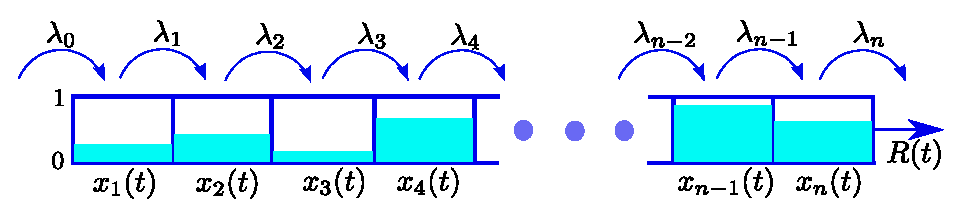
\includegraphics[width=.8\linewidth]{fig/rfm-diagram-hist.eps}
	\caption[Ribosome flow model]{A visual represenation for \acf{RFM}.}
	\label{fig:rfm}
\end{figure}

In the context of mRNA translation, the~$\lambda_i$'s depend on various biomechanical properties for example the abundance of tRNA molecules that deliver the amino-acids to the ribosomes. 
A recent paper suggests  that cells vary their~tRNA abundance in order to control the translation rate~\cite{Torrenteaat6409}. 

Note that if  ~$\lambda_k$ is   small for some~$k$ then the flow from site~$k$ to site~$k+1$ will be small, so site~$k$ fills up, that is~$x_k(t)$ will be close to one for all~$t$ sufficiently large. 
Consequently, the flow~$\lambda_{k-1} x_{k-1}  (1-x_{k} )$ from site~$k-1$ to site~$k$ will become small and then site~$k-1$ fills up. 
In this way, a traffic jam may evolve behind a ``bottleneck'' site.
The implications of such traffic jams in various biological transport processes is recently attracting  considerable interest (see, e.g.~\cite{tuller_traffic_jams2018,neurojams}).

It has been shown~\cite{margaliot2012stability} that there exists a unique~$e=e(\lambda_0,\dots,\lambda_n) \in(0,1)^n$ such that  any solution of the~\ac{RFM}  emanating from  the unit cube converges to~$e$. 
Thus, the system is globally asymptotically  stable. In particular, the production rate converges to the steady-state value 
\begin{equation}
	R:=\lambda_n e_n. 
\end{equation}

Ref.~\cite{rfm_concave} derived a spectral representation for the steady-state density~$e$ and production rate~$R$. 
Given the~\ac{RFM}, define the~$(n+2)\times(n+2)$ tridiagonal matrix:
%
\begin{align} \label{rfm:matrix}
B :=\begin{bmatrix}
	0 &  \lambda_0^{-1/2}   & 0 &0 & \dots &0&0 \\
	\lambda_0^{-1/2} & 0 & \lambda_1^{-1/2}   & 0  & \dots &0&0 \\
	0& \lambda_1^{-1/2} & 0 &  \lambda_2^{-1/2}    & \dots &0&0 \\
	& &&\vdots \\
	0& 0 & 0 & \dots &\lambda_{n-1}^{-1/2}  & 0 & \lambda_{n }^{-1/2}     \\
	0& 0 & 0 & \dots & 0 & \lambda_{n  }^{-1/2}  & 0
\end{bmatrix}.
\end{align} 
%
Note that~$B$ is (componentwise) nonnegative and irreducible.
Let~$\sigma>0$ [$\zeta \in \mathbb R^{n+2}_{>0}$] denote the Perron root [Perron vector] of~$B$ (see e.g.~\cite{matrx_ana}). 
Then
%
\begin{equation}\label{eq:rstar}
	R=\sigma^{-2} \text{ and } 
	e_i=\frac{  \zeta_{i+2} }{  \lambda_{i }^{1/2}    \sigma     \zeta_{i+1} } , \; i=1,\dots,n. 
\end{equation}
%
In other words, the steady-state values can be determined without any numerical simulations of the dynamics but rather using (efficient and numerically stable) algorithms for determining the Perron root and vector of tridiagonal matrices. 
Note that it follows from~\eqref{eq:rstar} that   
\begin{equation}
	R(c\lambda_0,\dots,c\lambda_n)=cR(\lambda_0,\dots,\lambda_n),\quad \text{ for all }c>0,
\end{equation}
that is, the steady-state production rate is positively homogeneous of degree one.


\subsection{Example}
\label{rfm:example}

Consider the~\ac{RFM} with all the rates equal to one. 
Then~$B$ is a tridiagonal Toeplitz matrix and it is well-known (see e.g.~\cite{spectral_toeplitz_tridiagonal}) that its eigenvalues are
%
\begin{equation}
	2\cos(\frac{k \pi}{n+3}) , \quad k=1,\dots,n+2,
\end{equation}
%
so the Perron root is~$\sigma=2\cos(\frac{  \pi}{n+3})$. 
The corresponding Perron vector is  
% 
\begin{equation}
	\zeta=\begin{bmatrix}  
		\sin(\frac{\pi  }{n+3}) &
		\sin(\frac{ 2 \pi  }{n+3}) &\dots&
		\sin(\frac{(n+2)\pi  }{n+3}) 
	 \end{bmatrix}^T. 
\end{equation}
%
Thus, in this case~\eqref{eq:rstar} gives
%
\begin{equation}
	\label{eq:rhom}
		R=\frac{1}{4}(\cos(\frac{  \pi}{n+3}))^{-2}
\end{equation}
%
and 
%
\begin{subequations}
	\begin{align} \label{eq:ehoms}
		e_i&=\frac{  \zeta_{i+2} }{      \sigma     \zeta_{i+1} } \\
		&=\frac{  \sin(\frac{ (i+2) \pi  }{n+3}) }{    2\cos(\frac{  \pi}{n+3})    \sin(\frac{ (i+1) \pi  }{n+3}) } 
	\end{align}
\end{subequations}
%
for all~$i=1,\dots,n$. 
For example, in the one-dimensional case, i.e.~$\dot x_1=1-2x_1$ it is clear that the equilibrium point is~$e=1/2$, so~$R=1/2$, whereas~\eqref{eq:rhom} yields 
%
\begin{equation}
R=\frac{1}{4}(\cos(\frac{  \pi}{4}))^{-2} = 1/2,
\end{equation}
%
and~\eqref{eq:ehoms} gives
%
\begin{equation}
e_1 = \frac{  \sin(\frac{ 3 \pi  }{4}) }{    2\cos(\frac{  \pi}{4})    \sin(\frac{ 2 \pi  }4) }  = 1/2.
\end{equation}
%

\subsection{Periodic excitation}

Biological organisms are exposed to periodic excitations like the 24h solar day and the periodic cell-cycle division  process. 
Proper functioning often requires entrainment to such excitations i.e. internal processes  must operate in a periodic pattern with the same period as the excitation. 
An example is the sleep-wake cycle that entrains to the 24h day. 

Ref.~\cite{entrainment} studied  the~\ac{RFM} with positive time-varying rates that are jointly~$T$-periodic, and proved that every state-variable~$x_i(t)$  converges to a periodic solution  with period~$T$.
In other words, the~\ac{RFM} entrains. 
The proof is based on the fact that the~\ac{RFM} is an (almost) contractive system~\cite{3gen_cont_automatica,cast_book}. 
However, this provides no information on the attractive periodic solution (except for its period). 
Obtaining  such information is a difficult problem (see~\cite{coogan_margaliot} and the references therein).

Since any set of jointly periodic rates induces a periodic solution, a natural  question is: can periodic rates yield  a higher production rate than constant rates? 
In this paper, we formulate this question rigorously, and show that it can be cast as an optimal control problem. 

\subsection{Bottleneck entrance}

In an analogous point of view, the~\ac{RFM} can be thought as a ``bottleneck entrance". 
And generalized to more applications like traffic systems, and scheduling at security checks with a cascade of an arbitrary Hurwitz positive linear system.
The cascade system etrains i.e. in response to a $T$-peridic inflow every solution converges to a unique~$T$-periodic solution of the system.
And, the objective would be to choose a periodic inflow rate with a given mean value that maximizes the average outflow rate of the system when maximizing the throughput is crucial. 

The  occupancy at time~$t$ in such applications can be modeled by the normalized state-variable~$x(t) \in [0,1]$.
In traffic systems,~$x(t)$ can be interpreted as the number of vehicles relative to the maximum capacity of a highway segment. 
For the security check, it is the number of passengers at a security gate relative to its capacity.
In  biological transport models discussed in the previous sections,  $x(t)$ is interpreted as the probability that a biological ``machine'' (e.g. ribosome,   motor protein) is bound to a specific segment of the ``trail'' it is traversing  (e.g. mRNA molecule, filament) at time~$t$.

The output in such systems is a nonnegative outflow which can be interpreted as the rate  of cars exiting the highway for the traffic system, or passengers leaving the gate for the security check.  
The inflow rates are often periodic, such as  those controlled by traffic light signals, or periodic flight schedules.  
Proper functioning often requires \emph{entrainment} to such excitations i.e. internal processes  must operate in a periodic pattern with the same period as the excitation~\cite{glass1979simple}. 
In this case, in response to a~$T$-periodic inflow the outflow converges to a~$T$-periodic pattern, and the \textit{throughput} is then defined as the ratio of the average outflow relative to the average inflow over the period~$T$.
  
As a general model for studying such applications is the cascade of two systems shown in Fig.~\ref{f.cascade}. 
The first block is called the \emph{bottleneck} and is given by:
\begin{subequations}
	\begin{align} \label{eq:con}
		\dot{x}(t) &= \sigma(t) (1-x(t)) - \lambda x(t),\\
		w(t)& = \lambda x(t),
	\end{align}
\end{subequations}
where $\sigma(t) >0$ is the inflow rate at time~$t$, $x(t) \in [0,1]$ is the occupancy of the bottleneck, and~$\lambda>0$ controls the output flow~$w(t)$. 
The rate of change of the occupancy is proportional to the inflow rate~$\sigma(t)$ and the \emph{vacancy}~$1-x(t)$, that is, as the occupancy increases the effective entry rate decreases.
\begin{figure}  
	\centering
	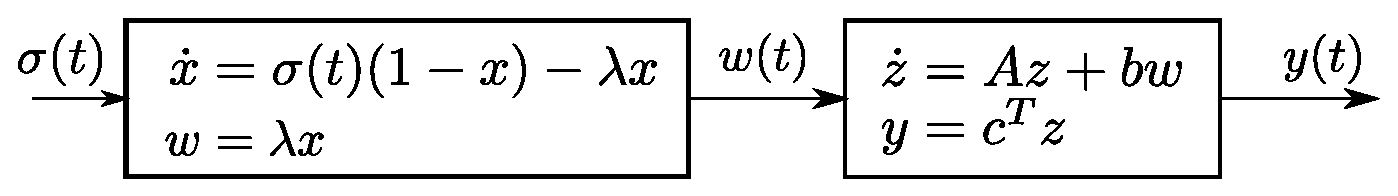
\includegraphics[width=0.8\columnwidth]{fig/rfm-cascade.eps}
	\caption[Cascade  system]{Cascade  system:  the bottleneck is feeding a positive linear system.}
	\label{f.cascade}
\end{figure}

A standard notation in this study.
Vectors [matrices] are denoted by small [capital] letters. 
For a vector~$x$, $x'$ denotes the transpose of~$x$. 
To follow the standard  practice of identifying any two measurable functions that are identical except perhaps on a set of measure zero.

Assuming that the inflow is periodic with period~$T\geq 0$, i.e. $\sigma(t+T)=\sigma(t)$ for all~$t\ge0$. 
The occupancy~$x(t)$ (and thus also~$w(t)$) entrains, as the system is  contractive~\cite{aminzare2014contraction,lohmiller1998contraction}. 
In other words, for any initial condition~$x(0)\in[0,1]$ the solution~$x(t)$ converges to a unique~$T$-periodic solution denoted~$x_\sigma$ and thus~$w $ converges to a~$T$-periodic solution~$w_\sigma$.

The outflow of the bottleneck is the input into  a Hurwitz    positive  linear system:
\begin{subequations}
	\begin{align} \label{linear_system}
		\dot z &= Az + b w ,\\
		y & =c^T z,
	\end{align}
\end{subequations}
where $A \in \mathbb R^{n\times n}$  is Hurwitz and Metzler and~$ b,c \in \mathbb R^n_+$ (see Figure~\ref{f.cascade}).
It is clear that for a~$T$-periodic~$\sigma(t)$, all trajectories of the cascade converge to a unique trajectory~$(x_\sigma(t),z_\sigma(t))$ with~$x_\sigma(t)=x_\sigma(t+T)$ and~$z_\sigma(t)=z_\sigma(t+T)$.

The objective for these applications is to compare the average (over a period) of~$y_\sigma(t)$ for various~$T$-periodic inflows. 
To make  a meaningful comparison, consider inflows that have a fixed mean~$\bar \sigma>0$, i.e 
\begin{equation}\label{average}
	\frac 1T \int_0^T \sigma(t) \diff t
	= \bar \sigma.
\end{equation}
The objective is maximize the gain of the system from~$\sigma$ to~$y$, i.e to maximize~$\int_0^T y_\sigma(t) \diff t $ for inputs with mean~$\bar \sigma$.

The trivial periodic inflow rate is the constant rate~$\sigma(t)\equiv \bar \sigma$. 
To compare the outflow  for this constant inflow with that obtained for an inflow that switches  between two values~$\sigma_1$ and~$\sigma_2$ such that $\sigma_2>\bar \sigma >\sigma_1>0$.
In other words,  $\sigma(t)\in \{\sigma_1,\sigma_2\}$ is periodic and satisfies~\eqref{average}.  

For the application in traffic system depicted in Figure~\ref{f.traffic}, there are two flows of vehicles with different rates~$\sigma_1,\sigma_2$ (e.g., cars and trucks) each moving in a separate road  and joining into a two-lane highway. 
This can be done in two ways. 
The first is to place traffic lights at the end of each road, and switch between them before entering the highway as in Figure~\ref{f.traffic}(a). 
The periodic traffic light signal~$\sigma(t)$ switches between the two flows, hence~$\sigma(t) \in \{\sigma_1,\sigma_2\}$. 
The second strategy is to have each road  constricted to a single lane, and then each joining the corresponding lane in the highway as in Figure~\ref{f.traffic}(b). 
Hence, the inflow rate is constant and equal to~$ (\sigma_1+\sigma_2)/2$. 
In both cases, the occupancy~$x(t)$ of the highway is modeled  by~\eqref{eq:con}. 
For a proper comparison, $\tfrac 1T \int_0^T \sigma(t) \diff t =   (\sigma_1+\sigma_2)/2$ as discussed before.
\begin{figure}[t!]
	\centering
	\begin{subfigure}[t]{0.9\textwidth}
		\centering
		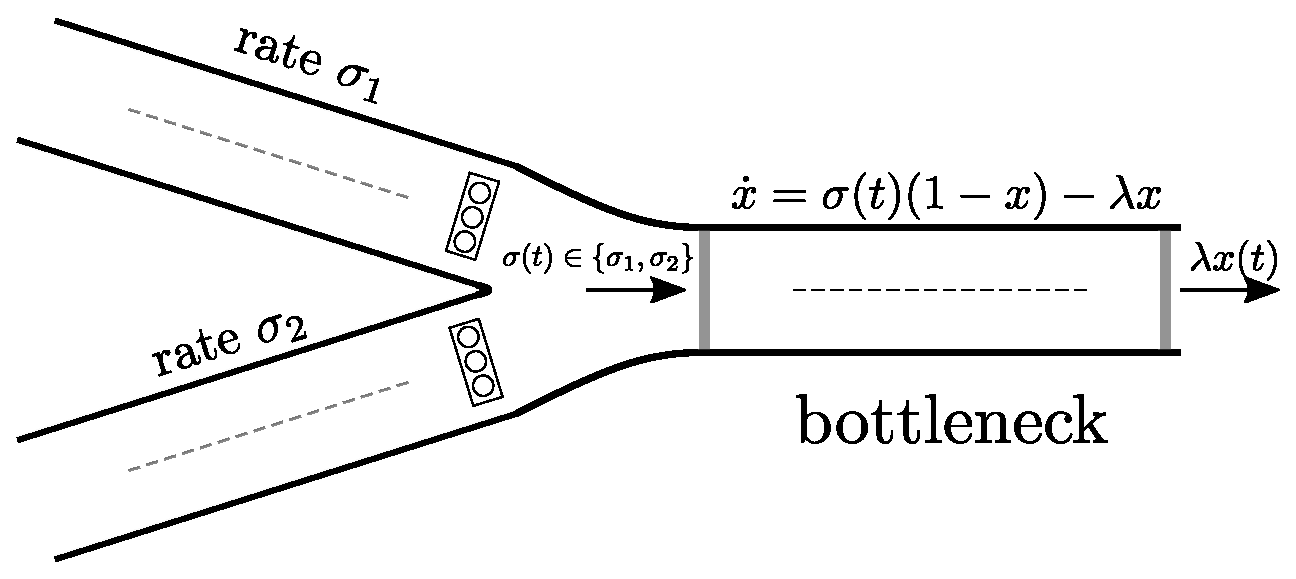
\includegraphics[width=\columnwidth]{fig/rfm-traffic-a.eps}
		\caption{}
	\end{subfigure}
	%
	\begin{subfigure}[t]{0.7\textwidth}
		\centering
		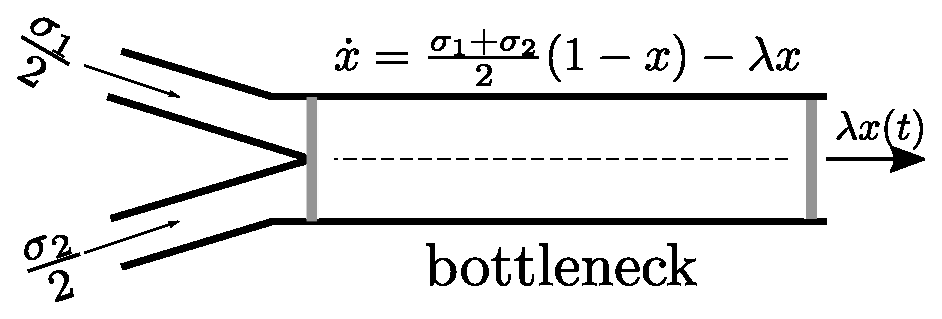
\includegraphics[width=\columnwidth]{fig/rfm-traffic-b.eps}
		\caption{}
	\end{subfigure}
	\caption[Traffic system illustration]{Traffic system application illustrating the two strategies.
		Here $x(t) \in[0,1]$  denotes the occupancy of the bottleneck at time~$t$. 
		(a)~The inflow rate switches via periodically-varying traffic lights between two flows with rates $\sigma_1,\sigma_2$. At each time, either vehicles in the upper lane or vehicles in the lower lane can enter the bottleneck, but not both. (b)~The double lane of each flow is restricted to a single lane and connected directly to the corresponding lane in the bottleneck. } 
	\label{f.traffic}
\end{figure}

\subsection{Problem Formulation}\label{sec:probform}

For any~$T$-periodic function~$f$, with~$T>0$, let~$\bar f:=\frac{1}{T}\int_0^T f(t)\diff t $, that is, the average of~$f$ over  a period. 
Pick a set of rates~$\lambda_i(t)$, $i=1,\dots,n$, that are jointly~$T$-periodic (note that a constant rate is~$T$-periodic for any~$T$). 
This induces a unique~$T$-periodic trajectory~$\gamma(t)$ of the~\ac{RFM} and thus a unique~$T$-periodic production rate~$R_T(t):=\lambda_n(t) \gamma_n(t)$~\cite{entrainment}. 
The average production rate is thus~$\overline {R_T}$. 
Consider an~\ac{RFM} with constant rates~$\overline { \lambda_i } $, $i=1,\dots,n$. 
Recall that every trajectory converges to a unique steady-state~$e$
and thus to a production rate~$R:=\overline { \lambda_n } e_n$. 

The question of interest in this study is: what is the relation between~$\overline {R_T}$ and~$R$?
Note that this is a ``fair'' comparison as we replace every time-varying rate by its average value. 

More generally, we can take a set of admissible rates~$S_{a,T}$ that are all jointly~$T$-periodic and satisfy~$\overline{\lambda_i}=a_i$.
Recall~$\sup_{S_{a,T}}  \{\overline {R_T}/R\}$, where the~$\sup$ is with respect to all the (non-trivial) rates in~$S_{a,T}$,  the \emph{periodic gain} of the~\ac{RFM}  over~$S_{a,T}$.
One can argue that the average production rate over a period, rather than the instantaneous  value, is the biologically relevant quantity.  
Then a periodic gain larger than one implies that we can ``do better'' using periodic rates. 
A periodic gain one implies that we do not ``loose'' anything with respect to the constant rates~$\lambda_i(t)\equiv a_i$.
A periodic gain smaller than one implies that for any (non-trivial) periodic rate the average production rate is lower than the one obtained for constant rates. 
This implies that entrainment  always incurs a cost, as the production rate for constant rates  is higher. 


\subsection{Structure of this chapter}
The remainder of this paper is organized as follows. 
Section~\ref{sec:simu} describes some simulation results for the general~\ac{RFM}.
Section~\ref{sec:optpercont} shows that the problem of finding the periodic gain can be cast as an optimal control problem. 
This implies that the  problem can be addressed using known and powerful tools from optimal control theory~\cite{pontryagin,LeeMarkus,liberzon}. 
By applying \ac{PMP} to analyze a particular case, namely, a one-dimensional~\ac{RFM} with a constant~$\lambda_1$ and a time-varying and periodic~$\lambda_0(t)$. 

%%%%%%%%%%%%%%%%%%%%%%%%%%%%%%%%%%%%%%%%%
\section{Numerical simulations} \label{sec:simu}

To gain a wider perspective, consider the case of a~\ac{SISO} asymptotically stable~\ac{LTI} system with input [output] $u(t)$ [$y(t)$] and transfer function~$G(s)$. 
Fix~$\omega,a>0$. 
Suppose that  the set of admissible inputs is
\[
\{    a+b\sin(\omega t):  b\in \mathbb R \}.
\]
Note that every input here is~$T$-periodic with~$T:=2\pi/\omega $, and that~$\overline u=a$. 
It is well-known that for~$u(t)=a+b\sin(\omega t)$ the output converges to~the~$T $-periodic function~$y_T(t):=|G(0)| a+|G(j\omega)| b   \sin(\omega t+ \angle G(j \omega))$, where~$j:=\sqrt{-1}$, so~$ \overline {y_T} =|G(0)| a  $. 
On the other-hand, if we replace~$u(t)$ by a constant input with value~$\overline u=a$ then the output converges to~$|G(0)| a$.
Thus, the periodic gain for this set of admissible inputs is one and by superposition it is one for any set of admissible~$T$-periodic inputs with average~$a$.  

Of course, for nonlinear systems, like the~\ac{RFM}, the periodic gain may be different than one. 
The next  example demonstrates this.

\subsection{Example} \label{subsec:sinsimp}
Consider the scalar system
\begin{equation} \label{eq:smsi}
	\dot x(t)= 1-x(t) u(t).
\end{equation}
%
For
%
\begin{equation} \label{eq:perub}
	u(t)=1 +(1/2) \cos(\omega t) ,
\end{equation}
%
with $\omega>0$, the solution is
%
\begin{equation}
	x(t)=\exp(-t-\frac{\sin(\omega t)}{2\omega } ) (x(0)+ \phi(t)) ,
\end{equation}
%
where~$\phi(t):=\int_0^t \exp(s+\frac{ \sin(\omega s)}{2\omega} ) \diff s$. 
%
In particular, for~$T:=2\pi/\omega$,
%
\begin{equation}
	x(T)=\exp(-T  ) (x(0)+ \phi(T) ).
\end{equation}
%
Now determine an initial condition~$x(0)=c$ for which the solution is~$T $-periodic, that is, 
%
\begin{equation}
	c=\exp(-T) (c+ \phi(T)),
\end{equation}
%
so
%
\begin{equation}
	c=\frac{\exp(-T) \phi(T)}{ 1-\exp(-T)}.
\end{equation}
%
Thus, the periodic solution is  $x_T(t):= \exp(-t-\frac{ \sin( \omega t)}{2\omega}  ) (c+ \phi(t)) $.
It is not difficult to show that this solution is attractive. 

On the other-hand, for a constant control with value~$\overline{u}=\frac{1}{T} \int_0^{T } u(s)\diff s=1$, the solution of~\eqref{eq:smsi} converges to the steady-state~$1$ and thus the periodic gain for the control~\eqref{eq:perub} is~$\overline {x_T}  = \frac{1}{T} \int_0^{T } x_T(t) \diff t $. 
Fig.~\ref{fig:sin} depicts~$\overline {x_T} $ as a function of~$\omega$. 
It may be seen that the periodic gain is always larger than~$1$, and that it approaches~$1$ as~$\omega \to \infty$. 

\begin{figure}[t!]
	\centering
	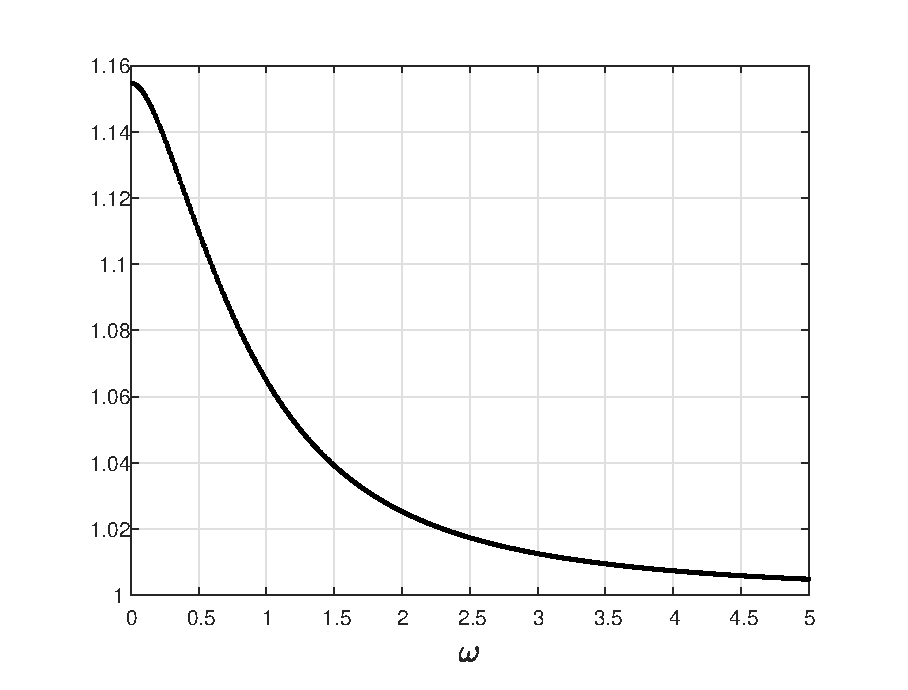
\includegraphics[width=.6\linewidth]{fig/exa_period_forcing.eps}
	\caption{Periodic gain in Example~\ref{subsec:sinsimp}
		as a function of~$\omega$.}
	\label{fig:sin}
\end{figure}

\subsection{Harmonic functions}
The~\ac{RFM} where  every rate is a sum of~$m$ harmonic functions  with random coefficients.
More precisely, we generated a matrix of random entries~$P \in \mathbb{R}^{(n+1)\times(2m)}$ and then set
%
\begin{align} \label{eq:rand} 
	\lambda_i(t) = 1 + \sum_{k=1}^{m} \left( p_{i, 2k-1} \sin(k \omega t) + p_{i, 2k} \cos(k \omega t)\right) , \qquad i=0,\dots,n. 
\end{align}
%
Note that this guarantees that the~$\lambda_i$'s are jointly~$T$-periodic for~$T=2\pi/\omega$ and that~$\overline{\lambda}_i=1$ for all~$i$. 
The entries of~$P$ are generated randomly with a uniform distribution over~$[-1/(2m), 1/(2m)]$, so  that~$\lambda_i(t)\geq 0$ for all~$i$ and all~$t$. 

The~\ac{RFM} with~$n=1$ is simulated first.
Since~$\overline {\lambda_i}=1$ for~$i=0,1$, and example~\ref{subsec:sinsimp}, it can be concluded that~$R=1/2$. 
Fig.~\ref{fig:1} depicts a histogram of the average steady-state flow~$\overline {R_T}$ for~$m=3$ and~$10,000$ random simulations.  
It may be seen that~$\overline{R_T}$ is always smaller than~$1/2$. Thus, the constant rates
yield the maximal  production rate. 

To explain this, consider the case where~$\lambda_1=1$ and~$\lambda_0(t)=1+\sin(\omega t)$.  
Let us compare this to the case where~$\lambda_1=1$ and~$\lambda_0= 1$. 
At times~$t$ such that~$\sin (wt)=-1$, there is less flow because~$\lambda_0(t)=0$.
At times~$t$ such that~$\sin(\omega t)=1$, there is more flow  because~$\lambda_0(t)=2$, but then~$\lambda_1$ becomes a bottleneck rate and slows down the flow, and thus on average we don't gain enough flow to compensate for what is lost.
This might be called the ``casino effect'': on average, the gains are not enough to compensate for the losses.

\begin{figure}[t!]
	\centering
	\begin{subfigure}[t]{0.49\textwidth}
		\centering
		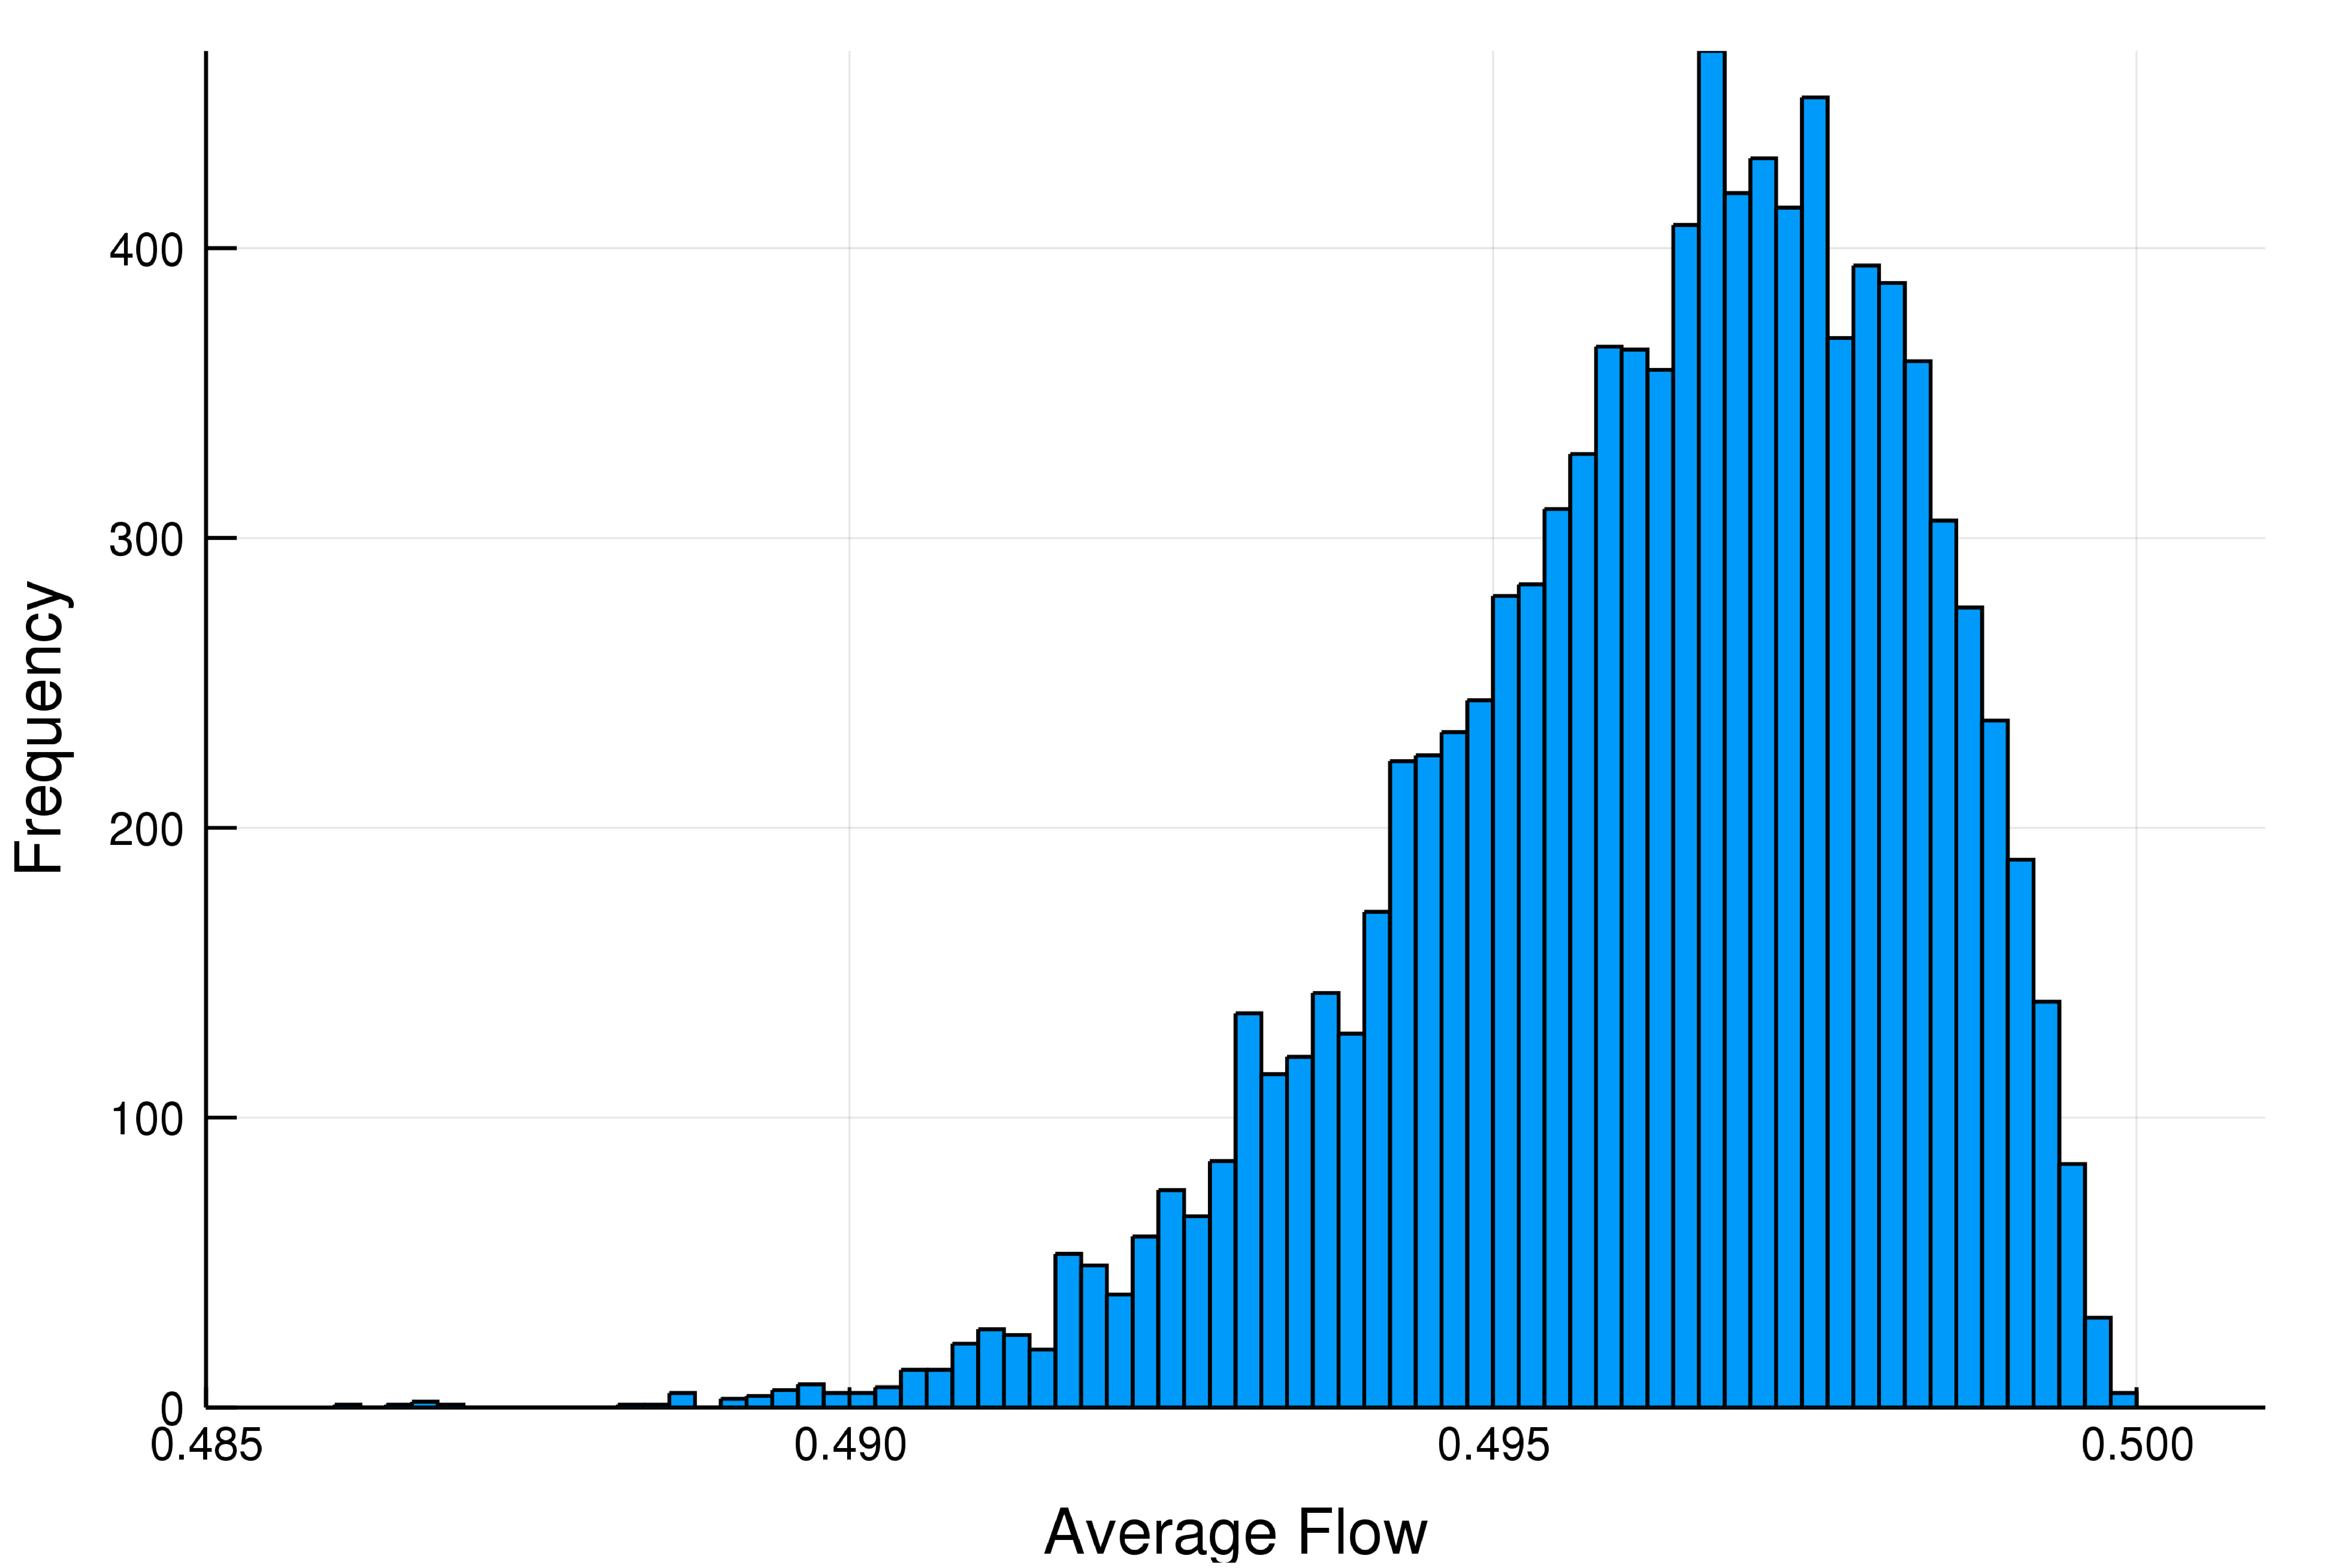
\includegraphics[width=.99\linewidth]{fig/rfm-hist1.eps}
		\caption{}
		\label{fig:1}
	\end{subfigure}
	%
	\begin{subfigure}[t]{0.49\textwidth}
		\centering
		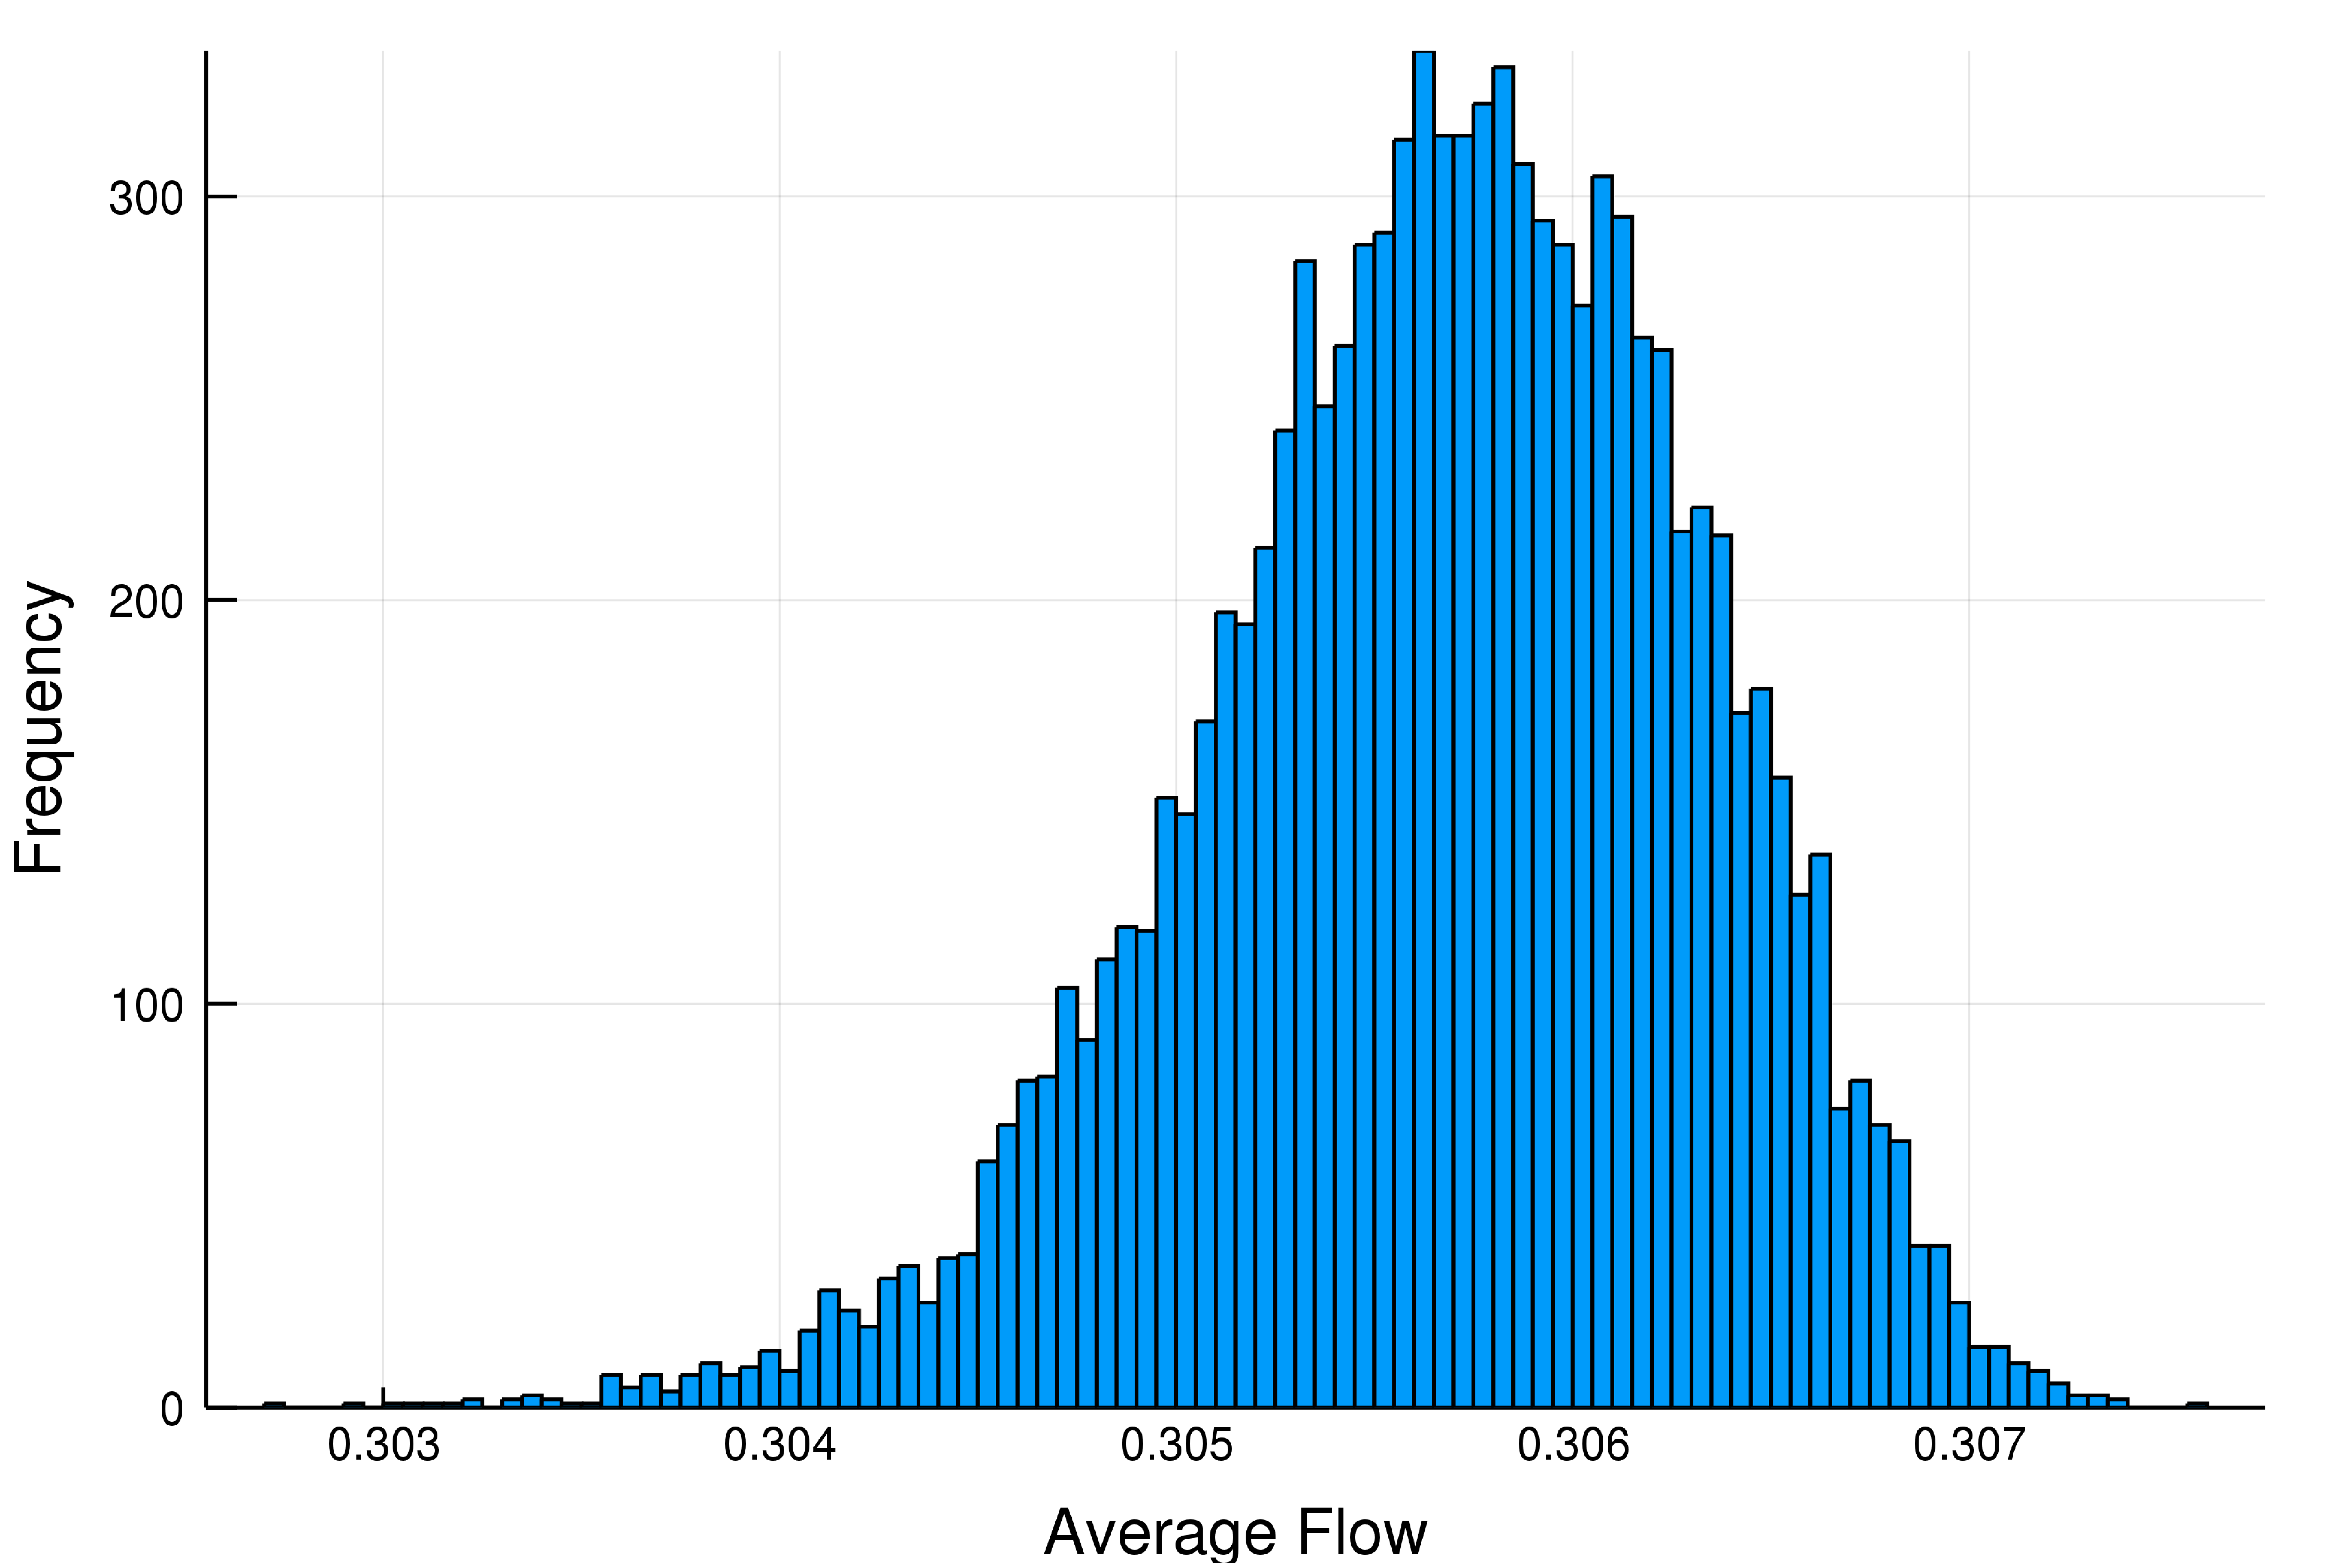
\includegraphics[width=.99\linewidth]{fig/rfm-hist2.eps}
		\caption{}
		\label{fig:2}
	\end{subfigure}
	\caption[Numerical simulations]{Numerical simulations: (a) A histogram of~$\overline{R_T}$ values 
		in the one-dimensional~\ac{RFM} with random
		periodic~$\lambda_0(t)$ and~$\lambda_1(t)$. 
		(b) A histogram of~$\overline{R_T}$ values 
		in an~\ac{RFM} with~$n=4$
		and periodic rates~$\lambda_i(t)$, $i=0,\dots,4$.}
\end{figure}

Consider now  an~\ac{RFM} with $n=4$ and constant rates set to one. 
By~\eqref{eq:rhom},
%
\begin{equation}\label{eq:ydcerp}
	R=\frac{1}{4}(\cos (  \pi/7))^{-2}\approx 0.307979.
\end{equation}
%
Fig.~\ref{fig:2} depicts a histogram representation of~$\overline{R_T}$ calculated over~$10,000$ simulations of an~\ac{RFM} with  random  periodic rates~$\lambda_0(t),\dots,\lambda_4(t)$.
It may be seen that~$\overline{R_T}$ is smaller than the value in~\eqref{eq:ydcerp}, so again the constant rates are those that maximize the production rate.  


%%%%%%%%%%%%%%%%%%%%%%%%%%%%%%%%%%%%%%%%%
\section{Optimal periodic control} \label{sec:optpercont}

The next goal is to pose the problem of determining the~\ac{RFM} periodic gain as an optimal control problem. 
The equations of the~\ac{RFM} can be augmented with an additional state-variable as follows 
%
\begin{subequations}\label{eq:rfm_aog}
	\begin{align}
		\dot z _1  &= \lambda_0 (1-z _1 )  - \lambda_1 z _1  (1-z _2 ), \\
		\dot z _k  &= \lambda_{k-1} z _{k-1}  (1-z _k )  - 
		\lambda_k z _k  (1-z _{k+1} ), \qquad 2\leq k \leq n-1, \\
		\dot z _n  &= \lambda_{n-1} z _{n-1}  (1-z _n )  - \lambda_n z_n ,\\
		\dot z_{n+1}&=\lambda_n z_n,\quad z_{n+1}(0)=0.
	\end{align}
\end{subequations} 
%
Thus,~$z(t)=\int_0^t R(\tau) \diff \tau$. 
Pick~$T>0$ and~$a_1,\dots,a_n>0$, and let~$S_{a,T}$ denote the set of measurable functions~$\lambda_i:[0,T]\to\mathbb{R}_+$ such that~$\overline{\lambda_i}=a_i$, $i=0,\dots,n$. 

By applying the spectral representation to determine  the steady-state production rate~$R$ when~$\lambda_i(t)\equiv a_i$ for all~$i$. 
Thus, determining the periodic gain is  equivalent to solving the following optimization problem.

\begin{problem} \label{prob:maxi}
	Maximize~$\frac{1}{T}z_{n+1}(T)$ over the set of admissible rates~$S_{a,T}$   with the boundary condition~$z_i(0)=z_i(T) \in (0,1)$ for~$i=1,\dots,n$.
\end{problem}
%
The last condition guarantees that we are maximizing  the production rate along the (unique) periodic trajectory. 
This optimal control problem can be addressed using known tools from optimal control theory~\cite{pontryagin,LeeMarkus,liberzon}. 
This special case can be demonstrated as follows.

\subsection{The case~$n=1$}

Pick~$T,a_0>0$, and consider the problem of computing the periodic gain of the one-dimensional~RFM with a constant~$\lambda_1>0$ and a time-varying~$\lambda_0:[0,T]\to \mathbb{R}_+$
with~$\overline{\lambda_0}=a_0$. 

Consider first the special  case where~$\lambda_0(t)$  is constant.
Then  clearly~$\lambda_0(t) \equiv a_0$, and thus
%
\begin{equation}
	\dot x_1=a_0(1-x_1)-\lambda_1 x_1.
\end{equation}
%
The steady-state of this equation is~$e_1=\frac{a_0}{a_0+\lambda_1}$, so~$\overline R=\frac{\lambda_1 a_0}{a_0+\lambda_1}$. 

To study the  case where~$\lambda_0(t)$ is not constant, it is useful to incorporate  the constraint~$\overline{\lambda_0}=a_0$ into the dynamics. 
Thus, the following system is considered. 
%
\begin{subequations} \label{eq:1rfm_e}
	\begin{align}
		\dot x_1(t)&=\lambda_0(t) (1-x_1(t)) -\lambda_1 x_1(t),  \\
		\dot x_2(t)&=\lambda_0(t),
	\end{align}
\end{subequations}
%
with the boundary conditions 
%
\begin{align} \label{eq:constr}
	x_1(T)=x_1(0),\;x_2(0)=0,\;    x_2(T)=T a_0. 
\end{align}
%
Fix~$L \geq 2 a_0 $. 
Determining the periodic gain is equivalent to solving the following problem.

\begin{problem} \label{prob:optim}
	Find $\lambda_0 : [0,T] \to [0,L]$ that maximizes the cost functional
	\begin{equation}
		J:=\frac{1}{T}\int_0^T \lambda_1 x_1(t) \diff t,
	\end{equation}
	subject to the dynamics~\eqref{eq:1rfm_e} and the boundary 
	conditions~\eqref{eq:constr}.
\end{problem}
%
The added bound on the size of~$\lambda_0(t)$ is needed because the presented solution in this study is using the~\ac{PMP}.

Note that the model~\eqref{eq:1rfm_e} can rewritten as a bilinear control  system.
%
\begin{equation}\label{eq:vec1rfm_e}
	\dot x=f(x)+g(x) u, 
\end{equation}
%
where~$u$ represents~$\lambda_0$,
$f(x):=\begin{bmatrix}
-\lambda_1 x_1 & 0 \end{bmatrix}' $,
and~$g(x):=\begin{bmatrix} 1-x_1 & 1\end{bmatrix}'$.
Thus, Problem~\ref{prob:optim} is a nonlinear optimal control problem (for other control problems for the~\ac{RFM}, see~\cite{zarai2018controllability}).  

The main result of this study can be stated as:
%
\begin{theorem}\label{thm:opt_struct}
	For any~$L\geq  2  a_0$ the unique solution of Problem~\ref{prob:optim} is the constant rate:
	\begin{equation}\label{optimal_u1} 
		\lambda_0^*(t) \equiv  a_0,
	\end{equation}
	and the corresponding optimal cost is:
	\begin{equation}
		J^*= \frac{\lambda_1 a_0}{\lambda_1+ a_0}.
	\end{equation}
\end{theorem}
%
Hence, the steady-state average flow of the system cannot be improved by using a periodic rate. 

The proof of Theorem~\ref{thm:opt_struct}  is based on applying the~\ac{PMP} to analyze the structure of optimal controls.

\subsection{Pontryagin's maximum principle for periodic trajectories} 

We apply the  \ac{PMP} to Problem~\ref{prob:optim}. 
The statement  of the \ac{PMP} in our case  is standard, except perhaps for the constraint that forces maximization over the periodic solution, i.e.~$x_1(0)=x_1(T)$.

Define the Hamiltonian 
%
\begin{subequations}
	\begin{align} \label{eq:hamiltonian}
		\mathcal H(u,x,p,p_0) &:= p' \left(f(x)+g(x) u  \right) 
		+\frac{1}{T} p_0 \lambda_1 x_1  \\
		&= (-p_1 \lambda_1  + p_0 \frac{1}{T} \lambda_1 ) x_1 
		+ (p_1(1-x_1)+p_2) u,
	\end{align}
\end{subequations}
%
where $p(t):=\begin{bmatrix} p_1(t)&p_2(t)\end{bmatrix}'$ is the adjoint, and $p_0\ge 0$ is called the abnormal multiplier.
Note that we can scale the Hamiltonian by scaling~$u$ and~$\lambda_1$. Thus, from here on we assume without loss of generality that~$\lambda_1=1$.

\begin{proposition}[PMP] \label{prop:pmp}
	Let $u^*(t):[0,T] \to [0,L]$ be an optimal control for 
	Problem~\ref{prob:optim}. Let~$x^*:[0,T] \to ([0,1] \times \mathbb{R}_+)$ be the corresponding optimal   trajectory. Let $p_0^*:=T $. There exists a
	function~$p^*: [0,T] \to  \mathbb{R}^2\setminus\{0\}$ such that:
	\begin{enumerate}
		\item The functions~$x^*(t)$ and $p^*(t)$ satisfy:
		\begin{subequations}
			\begin{align} \label{pdot}
				\dot  x^* & = \frac{\partial \mathcal H}{\partial p}(u^*,x^*,p^*,p_0^*) , \\ 
				\dot  p^* & = -\frac{\partial \mathcal H}{\partial x}(u^*,x^*,p^*,p_0^*);
			\end{align}
		\end{subequations}
		%
		\item The control $u^*(t)$  satisfies
		\begin{equation}\label{eq:pmp_max}
			\mathcal H(s,x^*(t),p^*(t),p_0^*) \le \mathcal H(u^*(t),x^*(t),p^*(t),p_0^*)
		\end{equation}
		for all $s \in [0,L]$  and almost every (a.e.)~$t \in [0,T]$ ;
		%
		\item The adjoint  satisfies the 
		transversality condition:
		\begin{equation} \label{eq:trans}
			p_1^*(0) = p_1^*(T).
		\end{equation}
	\end{enumerate}
\end{proposition}

A few remarks will be discussed before proving Proposition~\ref{prop:pmp}. 
First, note that~\eqref{pdot} yields
\begin{equation}
\dot p_1^*=	  (1+u)p_1^*-1,
\quad 	\dot p_2^*=0.
\end{equation}
so~$p_2^*(t)\equiv p_2^*(0)$. 
Second, define the \emph{switching function}~$\varphi^*:[0,T]\to\mathbb{R}$ by
%
\begin{subequations}
	\begin{align}\label{switching_function}
		\varphi^*(t)&:= (p^*(t))' g(x^*(t))\\&=
		p_1^*(t) (1-x_1^*(t)) + p_2^*(0).
	\end{align}
\end{subequations}
%
Note that~$\varphi^*(t)$ is absolutely continuous. 
Then~\eqref{eq:pmp_max} implies that
\begin{equation}\label{eq:ubang}
	u^*(t) = \begin{cases}
		L, & \varphi^*(t)>0,\\
		0, & \varphi^*(t)<0.
	\end{cases}
\end{equation}

A calculation yields
%
\begin{subequations}
	\begin{align} \label{phidot}
		\dot \varphi^*  &= \dot p_1 ^*(1-x_1^*) - p_1^* \dot x_1^*\\
		&= p_1^*   - 1+ x_1^* ,  \\
		\ddot\varphi^*  & =  \dot p_1^*+\dot x_1^* \\
		&=  ( 1-x_1^* +   p_1^*) u-   1-x_1^*+ p_1^*  . 
	\end{align}
\end{subequations}
%
Note that this implies that~$\dot\varphi^* $ is absolutely continuous, so~$\varphi^*  \in C^1$. 

\begin{proof}[Proof of Proposition~\ref{prop:pmp}]
	Most of the statements here are the standard~\ac{PMP}. 
	It is only necessary to prove  the transversality condition~\eqref{eq:trans}, and that~$p_0^*\not =0$. 
	
	Pick~$S\subseteq  \mathbb{R}^4$, and suppose that the state must satisfy the  constraint~$ \begin{bmatrix} x(0) & x(T) \end{bmatrix}' \in S$. 
	Then the transversality condition~\cite{LeeMarkus} is
    %
	\begin{equation}
	\begin{bmatrix} p(0) \\ -p(T) \end{bmatrix} \bot \mathcal T_{  \begin{bmatrix} x(0) \\ x(T) \end{bmatrix} } S, 
	\end{equation}
	%
	where $\mathcal T_{z } S$ is the  tangent space 
	of~$S$ at~$z $.
	In this case, $S = \{ z \in \mathbb{R}^4 | z_1-z_3=0, z_2=0, z_4=T a_0\}$. 
	Hence, $T_z S=\mbox{span}\{[1,0,1,0]'\}$.
	Therefore, it is necessary that $p_1^*(0)=p_1^*(T)$.
	
	Next  we show that the abnormal multiplier is not zero.
	Assume that~$p_0^*=0$. Then~\eqref{pdot} yields~ 
	%	
	\begin{equation}
	\dot  p_1^* = (1+u^* ) p_1^*.
	\end{equation}
	%
	Thus,~$p_1^*(t)\geq \exp(t) p_1^*(0)$ for all~$t\geq 0$. 
	If~$p_1^*(0)\not =0$ then this contradicts~\eqref{eq:trans}, so we conclude that~$p_1^*(0)=0$ and thus~$p_1^*(t) \equiv 0$. 
	This implies that~$p_2^*(0)\not =0$, and thus~\eqref{switching_function} and~\eqref{eq:ubang} imply that~$u^*(t)$ is constant. 
	But in this case it is clear that~$u^*(t)\equiv a_0$. 
	It can be concluded that by assuming~$p_0^*\not=0$, and by scaling the result is $p_0^*=T$.
\end{proof}


\subsection{The structure of an optimal control}

Given an optimal control~$u^*$, let
\begin{subequations}
	\begin{align}
		E_+^* :=\{ t \in [0,T]:  \varphi^*(t)>0\} , \\
		E_-^* :=\{ t \in [0,T] : \varphi^*(t)<0\},\\
		E_0^* : =\{ t \in [0,T] :  \varphi^*(t)=0\}.
	\end{align}
\end{subequations}
Note that all these  sets are measurable.

The next result analyzes singular arcs. 
For a measurable set~$F\subseteq [0,T]$, we use~$\mu(F)$ to denote the  Lebesgue measure of~$F$. 

\begin{lemma}\label{lemma:singular}
	Suppose  that~$u^*$ is an optimal control such that~$\mu(E_0^*)>0$.
	Then there exists a unique~$c_0\in ( 0,L]$ such that 
	\begin{equation} \label{singular}
		u^*(t)   \equiv  c_0  
		\text{ for a.e. }   t\in E_0 ^*, 
	\end{equation}
	and 
	\begin{equation}
		x_1^*(t)\equiv  \frac{c_0}{1+c_0} \text{ for all }  t \in E_0^*.
	\end{equation}
\end{lemma}

\begin{proof}
	Let $E^* \subseteq E_0^*$ denote  the set of accumulation points of~$E_0^*$.
	Note that~$\mu(E^*)=\mu(E_0^*)$, since $E_0^*-E^*$ is the set of isolated points of~$E^*$ which is countable, and hence has measure zero. 
	For~$t\in E^*$, we have $\varphi^*(t)=0$, so~$(\varphi^*(t) )^{(k)}:= \frac{d^k}{dt^k} \varphi^*(t) =0$ for any integer~$k\geq 0$.
	
	The equation~$\varphi^*(t)=\dot\varphi^*(t)=0$ yields~$p_1^*(t) (1-x_1^*(t)) \equiv -p_2^*(0)$, and $p_1^*(t) \equiv 1-x_1^*(t)$. 
	It can be concluded that 
	\begin{equation} \label{eq:xqpo}
	p_1^*(t)\equiv 1-x_1^*(t) \equiv r , 
	\end{equation}
	where $r$ is a constant. Since $x^*(t)\in (0,1)$,  $r\in (0,1)$. 
	Hence, $p_2^*(0) = -r^2 <0$.
	
	Combining~\eqref{eq:xqpo} 
	with  the fact that~$\ddot\varphi^*(t)=0$ yields
	\begin{equation}
		u^*(t) \equiv c_0,
	\end{equation}
	where~$c_0:=\frac{1-r}{r} $. Note that since~$u^*(t)\leq L$, 
	\begin{equation} \label{eq:blr}
		r(1+L)\geq 1 .
	\end{equation}
	%
	Now~\eqref{eq:xqpo}  yields~$x_1^*(t)\equiv 1-r=\frac{c_0}{1+c_0}$.
\end{proof}

Note that if~$r(1+L)=1$ then on any singular arc we have~$u^*(t)=c_0=L$.
This case is ``not interesting'' as then we can identify the singular arc with a bang arc. 
Thus from here on the assumption is that
\begin{equation}\label{eq:cnabh}
r(1+L)>1 .
\end{equation}

The notation~$B$ [$S$] is used to denote a bang [singular] arc. 
The bang arc can be either~$B_+$ (i.e.~$\varphi^*(t)>0$ on the arc), or~$B_{-}$.
The next result considers the concatenation of singular  and bang  arcs. 
\begin{proposition}
	An optimal control~$u^*$  cannot  contain a concatenation of    arcs in the form~$SBS$.
\end{proposition}

\begin{proof}
	Suppose that~$u^*$ includes a concatenation~$SBS$.  
	It is already known that there exists a unique value~$r$ such that~$x_1^*(t)\equiv 1- r$ and~$p_1^*(t)\equiv  r$ on both singular arcs. 
	
	Suppose that~$B=B_-$.
	Then~$\dot x_1^*= -x_1^*$ along the bang arc, so~$x_1^*(t)$ strictly  decreases on~$B_{-}$.
	But this is a contradiction, as~$x_1^*(t)$ must have the same value on both singular arcs. 
	
	
	Suppose now that~$B=B_+$.
	Then
	\begin{equation} \label{eq:pqlod}
		\dot p_1^*=(1+L)p_1^* -1^*
	\end{equation}
	along the bang arc.
	In particular, at the initial  time~$\tau \in(0,T)$ of~$B_+$, 
	\begin{equation}
		\dot p_1^*(\tau)=(1+L) r  -1^*
	\end{equation}
	and~\eqref{eq:cnabh} yields~$\dot p_1^*(\tau)>0$. 
	Combining this with~\eqref{eq:pqlod} implies that~$p_1^*(t)$ strictly increases on~$B_+$ and this is again a contradiction.
\end{proof}

The next result analyzes optimal controls that include two consecutive bang arcs.  
\begin{lemma}\label{lem:bnatr}
	An optimal control~$u^*$ cannot include any of the following concatenations:~$B_-B_+B_-$, $B_- B_+  S$,
	$B_+ B_- B_+ $, and~$B_+ B_- S $.
\end{lemma}

\begin{proof}
	Suppose that~$u^*$ includes~$B_+B_-$.
	Then there exists~$\tau \in(0,T)$ such that~$\varphi^*(t)>0$ for~$t\in (\tau-\varepsilon,\tau)$, and~$\varphi^*(t)<0$ for~$t \in (\tau,\tau+\varepsilon)$, with~$\varepsilon>0$.
	Hence~$\varphi^*(\tau)=0$ and~$\dot \varphi^*(\tau)\leq 0$. 
	Combining this with~\eqref{phidot} yields
	\begin{equation} \label{eq:ztrpp}
		\ p_1^* (\tau)   - 1+ x_1^*  (\tau) \leq 0 . 
	\end{equation}
	For any~$t \in ( \tau,\tau+\varepsilon) $  it is true that~$u^*(t)=0$, so $\dot x_1^*(t)=-x_1^*(t)$ and~$\dot p_1^*(t) = p_1^*(t)-1 $. 
	Thus,
	\begin{subequations}
		\begin{align}
			x_1^*(t)&= \exp(-(t-\tau)) x_1^*(\tau), \\
			p_1^*(t)&=1+\exp(t-\tau)(p_1^*(\tau)-1).
		\end{align}
	\end{subequations}
	Substituting this in~\eqref{phidot} yields
	\begin{subequations}
		\begin{align}
			\dot \varphi^*(t)
			&= \exp(t-\tau)(p_1^*(\tau)-1)+ \exp(-(t-\tau)) x_1^*(\tau)\\
			&<\exp(t-\tau) \left (  p_1^*(\tau)-1  +  x_1^*(\tau) \right ) ,
		\end{align}
	\end{subequations}
	where the last equation follows from the fact that along the periodic solution~$x_1^*(s)\in (0,1)$ for all~$s$. 
	Combining this with~\eqref{eq:ztrpp} implies that
	\begin{equation}
	\dot \varphi^*(t) <0 \text{ for all } t \in (\tau,\tau+\varepsilon).
	\end{equation}
	This clearly  implies that~$\varphi^*(t)<0$ for all~$t\in(\tau,T]$.
	Thus, the concatenations~$B_+B_-S$ and~$B_+B_-B_+$ are not possible.
	A similar argument shows that if~$u^*$ includes~$B_- B_+$ then the concatenations~$B_ - B_+ S$ and~$B_- B_ + B_-$ are not possible.
\end{proof} 

The analysis above implies that the most general form possible for an optimal control is
\begin{equation} \label{eq:mosyfr}
	B_1 S B_2 B_3,
\end{equation}
where every~$B_i$ stands for wither~$B_-$ or~$B_+$. 
Our  next goal is to compare a control~$u$ with such a structure to the control that includes a single singular arc. 
To do this, it is necessary to explicitly compute and compare the cost~$J$ along such controls. 
The following lemma is used in the solution of a scalar switched system. 
%
\begin{lemma}\label{lem:vsimprr}
	Pick~$b_1>b_2>0$ and~$a_1,a_2 \in \mathbb{R}$.  
	Suppose that starting  from~$y(0)=y_0$ and follow the dynamics~$\dot y=a_1  -b_1  y$ for~$t\in[0,t_1]$, with~$t_1>0$, and then switch to~$\dot y=a_2   -b_2  y$ for~$t\in [t_1,t_1+t_2]$, with~$t_2>0$,  and such that~$y(t_1+t_2)=y_0$  (that is, the system returns to its initial state).
	Then
		\begin{equation}\label{eq:redp}
			\int _{0}^{t_1+t_2} y(t) \diff  t <
			t_1 c_1+t_2 c_2
			+ \frac{t_1 t_2 (b_1-b_2)(c_1-c_2)}{b_1 t_1+b_2 t_2},
		\end{equation}
	where~$c_i:=a_i/b_i$.
\end{lemma}

\begin{proof}
	First consider the scalar equation~$\dot y=a -by$, with~$b\not =0$,~$y(t_0)=y_0$ and~$y(t_1)=y_1$. 
	Then integration yields
	\begin{equation}
		y_1-y_0=\int_{t_0}^{t_1} (a-by(t))\diff t=
		a(t_1-t_0)-b \int_{t_0}^{t_1} y(t) \diff t, 
	\end{equation}
	so
	\begin{equation} \label{eq:scalary}
	\int_{t_0}^{t_1} y(t) \diff t= (t_1-t_0)\frac{a}{b}-\frac{y_1-y_0}{b}. 
	\end{equation}
	
	Now fix~$b_1>b_2>0$.
	Suppose that starting  from~$y(0)=y_0$ we follow the dynamics~$\dot y=a_1  -b_1  y$ for~$t\in[0,t_1]$, with~$t_1>0$,   
	and then switch to~$\dot y=a_2   -b_2  y$ for~$t\in [t_1,t_1+t_2]$, with~$t_2>0$, 
	such that~$y(t_1+t_2)=y_0$.  
	That is, the system returns to its initial state.
	Then
	\begin{subequations}
		\begin{align} 
			y(t_1)&= c_1(1-\exp(-b_1 t_1) )+ \exp(-b_1 t_1)y_0    ,\\
			y(t_1+t_2)  &=c_2 (1-\exp(-b_2 t_2) )+ \exp(-b_2 t_2)y(t_1) , 
		\end{align}
	\end{subequations}
	where~$c_i:=a_i/b_i$. 
	Denoting~$y_1:=y(t_1)$ and using the fact that~$	y(t_1+t_2)=y_0$ yields 
	\begin{subequations}
		\begin{align} 
			y_1&= c_1(1-\exp(-b_1 t_1) )+ \exp(-b_1 t_1) \left(  c_2 (1-\exp(-b_2 t_2) )+ \exp(-b_2 t_2)y_1  \right)     ,\\
			y_0  &=c_2 (1-\exp(-b_2 t_2) )+ \exp(-b_2 t_2) \left ( 
			c_1(1-\exp(-b_1 t_1) )+ \exp(-b_1 t_1)y_0
			\right)  , 
		\end{align}
	\end{subequations}
	so
	\begin{equation}
	y_1-y_0= (c_1-c_2) \frac{(1-\exp(-b_1 t_1 ) )(1-\exp(-b_2 t_2 ) )   }{1-\exp(-b_1 t_1-b_2 t_2  ) } .
	\end{equation}
	It is straightforward to show that for any~$v,w>0$ we have
	\begin{equation}
	\frac{(1-\exp(-v))(1-\exp(-w))}{1-\exp(-(v+w))} <\frac{vw}{v+w},
	\end{equation}
	so we obtain the bound
	\begin{equation} \label{eq:bosdcu}
	y_1-y_0<  (c_1-c_2) \frac{ b_1 b_2 t_1 t_2   }
	{ b_1 t_1 + b_2 t_2  } .
	\end{equation}
	
	On the other-hand,~\eqref{eq:scalary} yields 
	\begin{subequations}
		\begin{align}\label{eq:odcp}
			\int _{0}^{t_1+t_2} y(t) \diff t&=
			\int_{0}^{t_1} y(t) \diff t + \int_{t_1}^{t_1+t_2} y(t) \diff t \\&
			= t_1 c_1-\frac{y_1-y_0}{b_1} 
			+ t_2  c_2-\frac{y_0-y_1}{b_2} \\
			&=t_1 c_1+t_2 c_2+(y_1-y_0)(b_2^{-1}-b_1^{-1}). 
		\end{align}
	\end{subequations}
	Using~\eqref{eq:bosdcu} and the fact that~$b_1>b_2>0$
	yields~\eqref{eq:redp} and this completes the proof.~\hfill{$\square$}
\end{proof}

The next result completes the proof of 
Theorem~\ref{thm:opt_struct}.
\begin{lemma}
	If~$u^*$ has the form~\eqref{eq:mosyfr} then~$u^*$ includes a single singular arc. 
\end{lemma} 

%%%%%%%%%%%%%%%%%%%%%%%%%%%%%%%%%%%%%%%%%
\section{A single stage RFM with two inputs}

Consider the scalar system with two inputs over a compact time interval $[0,T]$:
\[ \dot x = u_0(t) (1-x(t)) - u_1(t) x(t),\] with the integral constraints $\int_0^T u_0 (t) dt= T \bar u_0, \int_0^T u_1 (t) dt= T\bar u_1$.  
The one-dimensional problem with integral constraints can be lifted to a three dimensional system with boundary conditions as follows:
\begin{subequations}
	\begin{align}\label{rfm2}
		\dot x_1(t)&=u_0(t) (1-x_1(t)) - u_1 x_1(t),  \\
		\dot x_2(t)&=u_0(t), \\ 
		\dot x_3(t)&=u_1(t).
	\end{align}
\end{subequations}
with the boundary conditions 
\begin{align} \label{boundary}
	x_1(T)=x_1(0),\;x_2(0)=0,\;    x_2(T)=T \bar u_0, \;  x_3(0)=0,\;    x_3(T)=T \bar u_1. 
\end{align}

Given two positive numbers $\ell,L$ with $\ell<L$, the optimal control problem can be stated as follows:
\begin{problem} \label{prob:optim2}
	Find $u_0, u_1 : [0,T] \to [\ell,L]$ that maximizes the cost functional
	\begin{equation}
	J:=\frac{1}{T}\int_0^T u_1(t) x_1(t) \diff t,
	\end{equation}
	subject to the dynamics~\eqref{rfm2} and the boundary conditions~\eqref{boundary}.
\end{problem}

The result can be stated as follows:
\begin{theorem}\label{prob2in}
	For any $\ell,L$ with ~$0<\ell\le\bar u_0/(\bar u_1+\bar u_0)\le L$, the optimal cost for Problem~\ref{prob:optim2}  is
	\begin{equation}\label{optimal_cost}
		J^*= \frac{\bar u_0}{\bar u_1+ \bar u_0}.
	\end{equation}
	and it can be achieved by the following inputs:
	\begin{equation}\label{optimal_u2} 
		u_0^*(t) \equiv  \bar u_0,  u_1^*(t)\equiv \bar u_1.
	\end{equation}
\end{theorem}

\begin{remark}
	The control inputs that achieve  the optimal cost are not unique, since if the two control inputs are coupled via the equation $u_0(t)/\bar u_0 \equiv u_1(t)/\bar u_1$ then system will be given by:
	\[\dot x_1(t) =  u_0(t) \left (1 -  \frac{\bar u_1+\bar u_0}{\bar u_0}x_1(t)\right ).\]
	Then any measurable function $u_0$ will achieve $J^*$ given in \eqref{optimal_cost}.
\end{remark}

\subsection{Pontryagin's maximum principle}

Consider Problem \ref{prob2in}, let the $p(t)=[p_1(t),p_2(t),p_3(t)]$ be the accompanying co-state vector. 
The associated Hamiltonian can be written as:
\begin{equation}\label{hamil} 
	\mathcal H = (p_1(t) (1-x_1(t) ) +p_2(t)) u_0(t)+ ( x_1(t)(1-p_1(t)) + p_3(t) )  u_1(t).  
\end{equation}

The time-evolution of the co-state is given by the following ODE:
\begin{equation}
	\dot p = \begin{bmatrix} (u_0(t)+u_1(t)) p_1(t) - u_1 (t)\\ 0 \\ 0 \end{bmatrix},
\end{equation}
with the boundary condition $p_1(0)=p_1(1)$.

Hence, two of the co-states are constants and are given by 
\begin{equation}
	p_2(t)\equiv p_2(0), p_3(t)\equiv p_3(0).
\end{equation} 

In what follows, let $\mathscr X:=(u_0^*(t),u_1^*(t),x^*(t), p^*(t))$ be an optimal trajectory.   We first state the following lemma:

\begin{lemma} \label{l.bounds}
	Let $\mathscr X$ be an optimal trajectory. Then $x_1^*(t), p_1^*(t)  \in ( \tfrac{\ell}{L+\ell}, \tfrac L{\ell+L})$ for all $t \in [0,T]$.
\end{lemma}

\begin{proof}
	For the sake of contradiction, assume that $x(0) > L/(L+\ell)$. Since $u_0,u_1 \in [\ell,L]$, the comparison principle  implies $\dot x (t) > 0 $ for all $t$. Hence $x(T)>x(t)$, which contradicts $x(T)=x(0)$. The argument can be repeated if $x(0)< \ell/(L+\ell)$. Hence $x(0)=x(T) \in ( \tfrac{\ell}{L+\ell}, \tfrac L{\ell+L})$. Now assume that $\exists t^* \in (0,T)$ such that $x(t^*) > L/{L+\ell}>x(T)$, the same argument shows that $x(t)>x(T)$ for all $t \in (t^*,T]$ which is a contradiction. The argument can be repeated if $x(t^*) < \ell /(L+\ell)$. A similar argument can be made to prove the corresponding statement for $p_1(t)$.  
\end{proof}

\subsection{Characterization of of regular arcs}

Rhere are two inputs, so there are two switching functions: 
\begin{subequations}
	\begin{align}
		\varphi_0(t)& = p_1 (1-x_1)+p_2(0) \\
		\varphi_1(t)&= x_1 (1-p_1) + p_3(0) . 
	\end{align}
\end{subequations}

A regular arc is one in which the switching functions do not vanish when evaluated at it.
Since the Hamiltonian is linear in the control input, then the optimal control is bang-bang when the switching function does not vanish. 
This is stated in the following the Lemma:
\begin{lemma} \label{l.bang}
	Let $\mathscr X$ be an optimal trajectory, then if $\varphi_i(t) \ne 0$, $i=0,1$ then:
	\begin{equation}
		u_i^*(t)= \left \{ \begin{array}{rl} L &:  \varphi_i(t) > 0 \\
			\ell &: \varphi_i(t)<0  \end{array} \right . ,
	\end{equation} 
	i.e, $u_i(t)$ is a bang-bang control when corresponding switching function does not vanish.
\end{lemma}

\begin{proof}
	Without loss of generality, let $i=0$.
	Let $\varphi_0(t)>0$, and let $u_0^*(t) <L$. 
	However,
	\begin{equation} 
		\footnotesize{
		\mathcal H(u_0^*(t),u_1^*(t),x^*(t),p^*(t)) = \varphi_1(t) u_1^*(t)+\varphi_0(t) u_0^*(t)<\varphi_1(t) u_1^*(t)+\varphi_0(t) L = \mathcal H(L,u_1^*(t),x^*(t),p^*(t)), 
	}
	\end{equation}
	which violates condition 3 in Proposition \ref{prop:pmp}. 
	Hence, $u_0^*(t)<L$ is not optimal. 
	The same argument can be applied when $\varphi_0(t)<0$, and also for $i=1$.
\end{proof}

\subsection{Characterization of of singular arcs}

Given an optimal trajectory $\mathscr X$, let
\begin{subequations}
	\begin{align}
	E_+^i:=\{ t \in [0,T]:  \varphi_i^*(t)>0\} , \\
	E_-^i :=\{ t \in [0,T] : \varphi_i^*(t)<0\},\\
	E_0^i : =\{ t \in [0,T] :  \varphi_i^*(t)=0\},
	\end{align}
\end{subequations}
where $i=0,1$. Note that all these  sets are measurable.

We also need the time derivatives of the switching functions:
\begin{subequations}
	\begin{align}
	\dot\varphi_0(t) &= u_1(t) ( p_1 - (1-x_1)) \label{dotphi0}\\
	\dot\varphi_1(t) &= u_0(t) (1-x_1-p_1). \label{dotphi1}
	\end{align}
\end{subequations}
Note that $\dot\varphi_0,\dot\varphi_1$ are bounded, and continuous almost everywhere. 
Note also that the $\mbox{sgn}(\dot\varphi_0(t))=-\mbox{sgn}(\dot\varphi_1(t))$, which will be used later.

In this subsection the interest is in the case with $\mu(E_0^i)>0$ for either $i=0$ or $i=1$.  
A few lemmas are provided to characterize the system behaviour in such case.

\begin{lemma}\label{l.s1}
	Let $\mathscr X$ be an optimal trajectory, and assume that  ~$\mu(E_0^i)>0$ for $i\in\{0,1\}$.
	Then there exists ~$c_i \in ( \tfrac{\ell}{L+\ell}, \tfrac L{\ell+L})$ such that 
	\begin{equation}
	x_1^*(t)\equiv  c_i \text{ for all }  t \in E_0^{i'}.
	\end{equation}
	where $E_0^{i'}$ is the set of accumulation points of $E_0^i$. 
	Furthermore, the two inputs must be satisfying the following relationship:
	\begin{equation}\label{inputs_coupled}
		u_0(t) \equiv \frac{c_i}{1-c_i}  u_1(t), t \in E_0^{i'}.
	\end{equation}
\end{lemma}

\begin{proof}
	Let $ E_0^{i'} \subseteq E_0^i$ denote  the set of accumulation points of~$E_0^{i}$.
	Note that~$\mu(E_0^{i,'})=\mu(E_0^i)$, since $E_0^{i}-E_0^{i'}$ is the set of isolated points of~$E_0^i$ which is countable, and hence has measure zero. 
	For~$t\in E_0^{i'}$, the $\varphi_i^*(t)=0$, so~$(\varphi^*(t) )^{(k)}:= \frac{d^k}{dt^k} \varphi^*(t) =0$ for any integer~$k\geq 0$. 
	
	W.l.o.g, let $i=0$, The equation~$\varphi_0^*(t)=\dot\varphi_0^*(t)=0$ yields~$p_1^*(t) (1-x_1^*(t)) \equiv -p_2^*(0)$, and $p_1^*(t) \equiv 1-x_1^*(t)$. 
	In conclusion
	\begin{equation} \label{eq:xqpo2}
	p_1^*(t)\equiv 1-x_1^*(t) \equiv 1- c_0 , 
	\end{equation}
	where $c_0$ is a constant. Since $x^*(t)\in (0,1)$,  $r\in (0,1)$. 
	Hence, $p_2^*(0) = -c_0^2 <0$. 
	The same argument can be repeated when $i=1$.
	
	Since $x_1(t)$ is constant, then $\dot x(t) \equiv 0$ and \eqref{inputs_coupled} follows.
\end{proof}

The results above leave the possibility that $c_0 \ne c_1$. 
The following lemma provides further restrictions. 

\begin{lemma}\label{l.s2}
	Let $\mathscr X$ be an optimal trajectory. Then:
	\begin{enumerate}
		\item If $\mu(E_0^0 \cap E_0^1) > 0$, then $E_0^{0'}=E_0^{1'}$, and $\exists c \in (0,1)$ such that $x(t)\equiv c$ when $t\in E_0^{0'}$.
		\item	If $\mu(E_0^0 \cap E_0^1) =0$, and $\mu(E_0^0)>0$. Then $\dot \varphi_1(t)\equiv  0$ and there exists a constant $\bar\varphi_1 \ne 0$ such that $\varphi_1(t)=\bar\varphi_1 \ne 0$ on $t \in E_0^{0'}$. A parallel statement hold be exchanging $i=0$ with $i=1$.
	\end{enumerate}
\end{lemma}
\begin{proof}The two statements can be proved as follows:
	\begin{enumerate}
		\item Let $c_0, c_1$ be given as in Lemma \ref{l.s1}. Since $\mu(E_0^0 \cap E_0^1) > 0$, then $c_0=c_1$, which also uniquely determines $p_2(0),p_3(0)$. 
		Hence, $E_0^{0'}=E_0^{1'}$.
		\item The assumptions imply that $\varphi_0^*(t)=\dot\varphi_0^*(t)\equiv0$ for $ t \in E_0^{0'}$. 
		Using \eqref{dotphi0},\eqref{dotphi1}, it can be written that $\dot\varphi_1(t)=0$ if $\dot\varphi_0(t)=0$. 
		Since $x(t), p_1(t)$ on $E_0^{0'}$ are constant hence $\varphi_1(t)\equiv \bar\varphi_1 := c_0^2 +\lambda_3(0)$.
	\end{enumerate}
\end{proof}

The last lemma shows that an optimal trajectory has two disjoint case for the singular arcs. 
Either each singular arc has both switching functions vanishing together, or only one of them can vanish at a time.

\subsection{Admissible Switching Patterns}
In the previous subsection we have shown that the optimal control can either be a bang-bang or singular. 
On the singular arc, the controls need to satisfy \eqref{inputs_coupled} but the state is constant, hence the value of the free input has no effect on the dynamics since $\dot x_1=0$ on all singular arcs.   
In general, there can be an arbitrary switching between these cases. 
In this part, the class of admissible switching patterns become more restricted. 

Assuming that control inputs are \textit{piecewise continuous}, and hence the switching functions are piecewise differentiable.  
An \emph{arc} is the restriction of the optimal trajectory $\mathscr X$ onto a maximal time interval such that the switching functions have a constant sign on that interval. 
Hence, the optimal trajectory $\mathscr X$ can be decomposed into a sequences of arcs. 

In order to facilitate the discussion we define the concept of an \emph{arc sign} as an ordered pair.  
An arc has a sign $s=(s_0,s_1) \in \mathscr S^2:= \{0,+,-\}^2$ iff $\mbox{sgn}(\varphi_i(t))\equiv s_i$ for $i=0,1$. Let $s^j,s^k$ be the signs of two consecutive arcs. 
An \emph{arc transition} is an ordered tuple  of arc signs, and is represented as follows: $s^j \to s^k$.  
The \emph{reverse} of an arc transition $s^j \to s^k$ is $s^k \to s^j$.  A switching transition is said to be \emph{inadmissible} if it can not occur in an optimal trajectory.

Some arc transitions are excluded in the following lemma:
\begin{lemma}\label{l.t1}
	Let $\mathscr X$ be an optimal trajectory. Then the following arc transitions and their reverses are inadmissible:  $(+,+) \to (-,-)$,  $(0,0) \to (+,+)$, $(0,0) \to (-,-)$. 
\end{lemma}

\begin{proof}
	Consider two consecutive arcs with a transition time $\tau$. 
	Hence, there exists $\varepsilon >0$ such that the first arc defined on a time interval $(\tau-\varepsilon,\tau)$ with sign $(+,+)$, and second arc defined on  $(\tau,\tau+\varepsilon)$ with sign $(-,-)$. Since both switching functions change sign from positive to negative at $\tau$, then we have $D_\tau^+ \varphi_i(t) \le 0, i=0,1$, where $D_\tau^+$ is the upper right Dini's derivative at $\tau$ \footnote{ $D_\tau^+ \varphi(t):=\limsup_{h \to 0^+} (\varphi(\tau+h)-\varphi(\tau))/h.$ }. 
	This also implies that $\exists \varepsilon_2 \le \varepsilon$ such that $\dot\varphi_i(t)<0$ for $t \in (\tau,\tau+\varepsilon_2), i=0,1$. 
	But this contradicts \eqref{dotphi0},\eqref{dotphi1} which imply that $\mbox{sgn}(\dot\varphi_0(t))=-\mbox{sgn}(\dot\varphi_1(t))$. 
	So this means that transition $(+,+) \to (-,-)$ can not be realized by any trajectory, including an optimal trajectory $\mathscr X$. \\
	A similar argument can be provided for all other cases.
\end{proof}

Let $(s_0,s_1)$ be the sign of an arc. 
An arc sign's entry $s_i$  is said to be \emph{locked} to $s \in \mathscr S$ if all subsequent arcs have signs with $s_i=s$. 
An arc sign's entry written as $\square{s}$ means that entry is locked to $s \in \mathscr S$. 
For example, an arc with the sign $(\square{+},-)$ means that all subsequent arcs have a sign of the form $(+,s)$ for some $s \in \mathscr S$.  
The notation $(s_0,s_1) \to (\square{s}, s^*)$  means that the transition result in  the first entry being locked to $s$. 
Similarly $(s_0,s_1) \to (s^*,\square{s})$ means that the second entry will be locked to $s$.

The following lemma is based on the notation introduced above:
\begin{lemma}
	Let $\mathscr X$ be an optimal trajectory, and consider two consecutive arcs.
	 Then $\forall s \in \mathscr S$, a transition of the form $(+,s) \to (-,+)$ is equivalent to  $(+,s) \to (\sq{-},+)$. 
	The parallel statements also hold with $(-,s) \to (\sq{+},-), (s,+) \to (+,\sq{-}), (s,-)\to(-,\sq{+})$.
\end{lemma}
\begin{proof}
	Consider the transition $(+,s) \to (-,+)$, and let $\tau$ be the transition time. 
	Then,  $\varphi_0(t)>0$ on $(\tau-\varepsilon_2,\tau)$ and $\varphi_0(t)<0$ on  $(\tau,\tau+\varepsilon_1)$, where $\varepsilon_1,\varepsilon_2>0$ are the duration of each of the two arcs, respectively.
	By Lemma \ref{l.bang}, we have $u_0(t)\equiv \ell, u_1(t) \equiv L$ for $t \in (\tau, \tau+\varepsilon_1)$. 
	Similar to the proof of the previous lemma, $D_\tau^+ \varphi_0 (t) \le 0$, which can be written as follows:
	%
	\begin{equation} \label{phi_ineq}
		D_\tau^+ \varphi_0 (t) = u_1(\tau_+) (p_1(\tau)-(1-x_1(\tau)) ) = L( p_1(\tau)- (1-x_1(\tau)) )  \le 0, 
	\end{equation}
	%
	Recall that $\dot x_1 = u_0 - (u_0+u_1)  x_1, \dot p = (u_0+u_1) p - u_1$.
	Following on $t \in (\tau,\tau+\varepsilon_1):$
	%
	\begin{subequations}
		\begin{align} \label{x_ineq}
			x(t) &= \left ( x(\tau) - \frac{\ell}{\ell+L} \right ) e^{-(\ell+L)(t-\tau)} + \frac {\ell}{\ell+L} < \left ( x(\tau) - \frac{\ell}{\ell+L} \right ) e^{(\ell+L)(t-\tau)} + \frac {\ell}{\ell+L}\\
			p(t) &= \left ( p(\tau) - \frac{L}{\ell+L} \right ) e^{(\ell+L)(t-\tau)} + \frac {L}{\ell+L},
		\end{align}
	\end{subequations}
	where the inequality \eqref{x_ineq} follows since $x(t)> \frac{\ell}{\ell+L}$ by Lemma \ref{l.bounds}.
	
	Consdiering the derivative of the switching function on $(\tau,\tau+\varepsilon_1)$ and use inequalities \eqref{x_ineq}, \eqref{phi_ineq} as follows:
	\begin{align}
		\dot\varphi_0(t) = L ( p_1(t) + x_1(t) - 1 )  < L ( x(\tau)+p(\tau) -1  ) e^{(\ell+L)(t-\tau)}  \le 0.
	\end{align}
	Hence, $\dot\varphi_0(t)<0$ on $(\tau,\tau+\varepsilon_1)$. 
	From $\varphi_0(\tau)=0$, and integrating 
	\begin{equation}
		\label{phi0_ineq} \varphi_0(t)<0  \ \mbox{for} \  t \in (\tau,\tau+\varepsilon_1). 
	\end{equation} 
	The claim is that this implies that $u_0(t)=\ell$ for $t \in (\tau, T]$.  
	The proof is: For the sake of contradiction assume that $u_0(\tau+\varepsilon_1)=L$. 
	By Lemma \ref{l.bang}, this is only optimal if $\varphi_0(\tau+\varepsilon_1)>0$ which  contradicts \eqref{phi0_ineq} since $\varphi_0$ is continuous. 
	Hence $(+,s_1) \to (-,+) \to (+,s_2)$ is not admissible for any $s_1,s_2 \in \mathscr S$. 
	Similarly,  $(+,s_1) \to (-,+) \to (0,s_2)$ is not possible since it violates continuity of  $\varphi_0$.  
	Hence $(+,s) \to (-,+)$ is equivalent to $(+,s) \to (\sq{-},+)$.\\ 
	Similar arguments can be repeated for the other cases.
\end{proof}

There are other transitions should be excluded. They are stated in the following two lemmas:
%
\begin{lemma}
	Let $\mathscr X$ be an optimal trajectory. 
	Consider two consecutive arcs.
	 The following transition is not admissible: $(+,0) \to (-,s)$,  for any $s \in \mathscr S$. Similarly, $(+,0) \to (0,s)$, $(-,0) \to (+,s)$, $(-,0) \to (0,s)$,  $(0,+) \to (s,-)$, $(0,+) \to (s,0)$,  $(0,-) \to (s,+)$ ,   $(0,-) \to (s,0)$ for any $s \in \mathscr S$. 
	 Also, all their reverses.
\end{lemma}
%
\begin{proof}   
	W.l.o.g, let's have the transition $(0,+) \to (+,0)$. 
	Let $\tau$ be the transition time. 
	There exists $\varepsilon >0$ such that $\varphi_1(t)\equiv 0 $ for $t \in (t,t+\varepsilon)$, and (by Lemma \ref{l.s2})  $\varphi_1(t) \equiv \bar\varphi_1 >0$ for $t \in (\tau-\varepsilon, \tau)$. 
	This implies that $\varphi_1(t)$ is discontinuous at $\tau$; a contradiction. 
	The same argument can be used for the other cases.
\end{proof}

\begin{lemma}
	Let $\mathscr X$ be an optimal trajectory, and consider three consecutive arcs. 
	Then, the following transition is  inadmissible: $(+,0) \to (+,+) \to (+,0)$. 
	Similarly, the following transitions are inadmissible $(0,+) \to (+,+) \to (0,+)$, $(-,0) \to (-,-) \to (-,0)$, $(0,-) \to (-,-) \to (0,-)$
\end{lemma}
%
\begin{proof}
	Let the arcs be defined on the following time intervals $(\tau_1-\varepsilon_1,\tau_1), (\tau_1,\tau_2), (\tau_2, \tau_2+\varepsilon_2) $ for some $\tau_1,\tau_2,\varepsilon_1,\varepsilon_2>0$. 
	Then on the first arc, Lemma \ref{l.s1} gives that $x_1(t)\equiv c_0$ for $t \in (\tau_1-\varepsilon_1,\tau_1)$. 
	On the second arc, the system is represented by $\dot x_1 = L(1-2x)$, with $x(\tau_1)=c_0$, and the third arc we have $x(\tau_2)\equiv c_0$ for $t \in (\tau_2,\tau_2+\varepsilon)$. 
	If $c_0 \ne \tfrac 12$, then it follows  $x_1$ is discontinuous at $\tau_2$; a contradiction. If $c_0=\tfrac 12$, then this implies that $x_1(t)\equiv c_0$ on the second arc which implies that $\varphi_0(t)\equiv 0$ on that arc, i.e it has a sign $(0,+)$; a contradiction. 
	The proof is similar for the remaining cases.
\end{proof}


Using Lemma \ref{l.s2}, If an optimal trajectory has an arc with the sign (0,0), then it can not have arcs with signs $(\pm,0)$ or $(0,\pm)$.
Using the above lemmas, there is no cycle possible amongst the arc signs. So,
%
\begin{proposition} \label{prop:17}
	Let $\mathscr X$ be an optimal trajectory. Then, it can not have more than 9 arcs.  
\end{proposition}
%
The proof consists of starting from an arc sign, and then tracing the longest possible arc transitions. All such paths will terminate, and the longest one can be found.
For instance,  if the optimal trajectory $\mathscr X$ has an arc with sign $(0,0)$, then the transition diagram is simple. 
If the trajectory starts from $(+,-)$ then the longest paths are as follows:
\begin{center}
	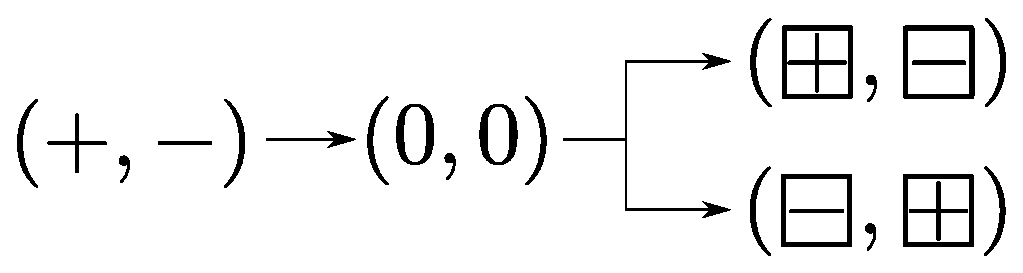
\includegraphics[width=0.35\textwidth]{fig/case_i.eps}
\end{center}
A similar diagram can be given if the trajectory starts from $(-,+)$. 
If it starts from $(+,+)$ or $(-,-)$ then $(0,0)$ cannot appear, and the diagram will be a subset of the diagram in the second case that follows.

The second case is when singular arcs can be present but without an arc with the sign $(0,0)$. The longest path diagram is as follows:

\begin{center}
	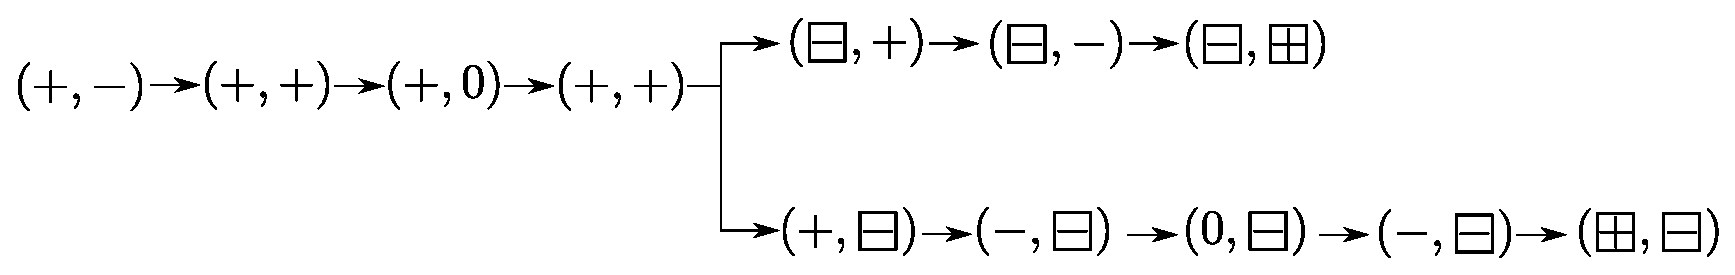
\includegraphics[width=\textwidth]{fig/case_ii.eps}
\end{center}

All other transitions that share the first two arcs are subsets of these longer transitions above. 
For instance, if the trajectory starts from any of the first three arcs to get a diagram, or it can eliminate the singular arcs from the diagram above to get admissible trajectories consisting entirely of regular arcs. Also, the second arc's sign can be changed to $(-,-)$ and a dual diagram can be given. 
Similar transition diagrams can be given when we start with $(-,+)$ instead.

\subsection{Suboptimality of admissible switching patterns}
%
In this part, longest path, given in the previous sections, are shown to be suboptimal.
 The following tricks helps to reduce the number of cases that were provided in Prop.~\ref{prop:17}.

\begin{lemma} \label{lemma:18}
	Any trajectory with $n$ arcs that is starting and ending with the same arc can be written with $n-1$ arcs without loss of generality.
\end{lemma}
%
\begin{proof}
	Consider a trajectory that starts with $(s_1, s_2)$ arc $t\in(0,\tau_1)$ and finishes with $(s_1, s_2)$ arc $t\in(T-\tau_2,T)$. 
	By defining the period between for $t\in(\tau_1,T+tau_1)$. 
	The trajectory starts with the 2nd arc at time $\tau_1$ and finishes at time $T+\tau_1$, where the last arc's time length is $\tau_1+\tau_2$.
\end{proof}

The following lemma, helps to derive one integral for the four optimal trajectories that were defined in Prop.~\ref{prop:17} and include an arc with sign $(0,0)$.
%
\begin{lemma} \label{lemma:19}
	If the optimal trajectory $\mathscr X$ has an arc with sign $(0,0)$, then it can be written in the form of $(+,-)\to(0,0)\to(-,+)$.
\end{lemma}
%
\begin{proof}
	From the Porp.~\ref{prop:17} and Lemma~\ref{lemma:18}, the optimal trajectory $\mathscr X$ that has an arc with sign $(0,0)$ can be written in the form of $(0,0)\to(-,+)$, $(0,0)\to(+,-)$, $(+,-)\to(0,0)\to(-,+)$, and $(-,+)\to(0,0)\to(+,-)$.  
	The $(0,0)\to(-,+)$, and $(-,+)\to(0,0)\to(+,-)$ trajectories contradict the periodicity of the optimal trajectory, while and $(+,-)\to(0,0)\to(-,+)$ is equivalent to $(-,+)\to(0,0)\to(+,-)$ by shifting the period to the starting time of the last arc of each trajectory. 
\end{proof}

Now, the cost function of Problem~\ref{prob:optim2} can be driven, for the optimal trajectory that was defined in lemma~\ref{lemma:19}. 
Consider that the $(+,-)$ arc switches to $(0,0)$ trajectory at $\tau_1$, then switches to $(-,+)$ at time $T-\tau_2$. 
The cost function would be: 
%
\begin{subequations}
	\begin{align}
		J :&=  \frac{1}{T}\int_0^{T} u_1(t) x_1(t) dt, \\
		&= \frac{1}{\tau_1}\int_0^{\tau_1} u_1(t) x_1(t) dt + \frac{1}{T-\tau_1-\tau_2}\int_{\tau_1}^{T-\tau_2} u_1(t) x_1(t) dt + \frac{1}{\tau_2}\int_{T-\tau_2}^{T} u_1(t) x_1(t) dt, \\
		&= c_0 \mu(E^0)  +c_+ \mu(E^+)   +c_- \mu(E^-)
		+     (c_+ - c_-)  ( {b_+} - {b_-}  ) 
		\sum_{i=1}^n \frac{  t_i^+  t_i^-  }{ b_+ t_i ^+ + b_- t_i^- }.
	\end{align}
\end{subequations}

Considering the \eqref{l.bang} values for $-$ and $+$ signs of the arc, and $c_0$, $c_1$ for the singular value sign $0$. 
The boundary conditions~\eqref{boundary} imply that:
\begin{subequations}
	\begin{align}
		\bar u_0 = \frac{L \tau_1 + c_0 (T-\tau_1-\tau_2) + l \tau_2}{T}, \\
		\bar u_1 = \frac{l \tau_1 + c_1 (T-\tau_1-\tau_2) + L \tau_2}{T}.
	\end{align}
\end{subequations}

%%%%%%%%%%%%%%%%%%%%%%%%%%%%%%%%%%%%%%%%%
\section{Conclusion}
If so, then may be we can call this the ``casino effect'' the gains are never enough to compensate for the losses.
This means that entertainment to a (non-trivial) periodic signal always incurs a cost, as the production rate would have been better for constant signals.


An interesting research direction is to prove that for certain general classes of contractive systems the periodic gain is one. 
This may be done for example by considering cases where the~PMP is not only a necessary condition for optimality, but also a sufficient condition. 

An interesting goal is to derive  a simple to test ad-hoc  procedure for determining whether the periodic gain is larger or smaller than one.  
A simple idea in this direction is for the case of a single periodic rate, say~$\lambda(t)$.
Suppose that for a constant rate~$\lambda(t)\equiv a$ the steady-state output is~$f(a)$. 
Suppose also that~$f\in C^2$, and that~$f'(a)> 0$. 
For~$\varepsilon>0$ sufficiently small, then
\begin{equation}
	f(a+\varepsilon)-f(a) \approx \varepsilon f'(a) +\frac{\varepsilon^2}{2} f''(a)   >0,
\end{equation}
i.e. when increasing~$a$ to~$a+\varepsilon$ we increase  the steady state-state  by~$\varepsilon f'(a) +\frac{\varepsilon}{2} f''(a)$. 
Similarly, 
\begin{equation}
f(a-\varepsilon)-f(a) \approx  -\varepsilon f'(a) +\frac{\varepsilon^2}{2} f''(a)   <0,
\end{equation}
i.e.  when decreasing~$a$ to~$a-\varepsilon$, to reduce the steady state-state by~$ \varepsilon f'(a)  - \frac{\varepsilon^2}{2} f''(a)$.
The ``total gain''  when~$a$ is varied in the range~$[a-\varepsilon,a+\varepsilon]$ is thus~$\varepsilon^2  f''(a)$.  
The same result is obtained when~$f'(a)<0$. 
This suggests that if~$f''(a)>0$ ($f''(a)<0$) then the ``total gain'' is positive [negative]  and it may be expected the periodic gain (for rates that vary around an average~$a$) to be larger [smaller] than one.

To demonstrate this, note that for the~RFM with~$n=1$ and~$\lambda=1$, the steady-state production rate~$R=f(\lambda_0)$  with
\begin{equation}
f(\lambda_0):=\frac{\lambda_0}{1+\lambda_0},
\end{equation}
so
\begin{equation}
f''(\lambda_0) =\frac{-2}{(1+\lambda_0)^3} <0,
\end{equation}
and this agrees with the fact that the periodic gain is smaller than one. 

On the other-hand, for the system in Example~\ref{exa:sinsimp}, for~$u(t)\equiv a$, with~$a> 0$, 
the output is~$f(a):=1/a $, so 
\begin{equation}
f''(a) = 2a^{-3}  > 0,
\end{equation}
and this agrees with the fact that the periodic gain is larger than one. 